% ============================================================
%  The Fertile Vacuum — Pitch Deck
%  Canva-style: bold colors, large type, minimal text, visual-first
% ============================================================
\documentclass[aspectratio=169,14pt]{beamer}

% --- Theme & Colors ---
\usetheme{default}
\setbeamertemplate{navigation symbols}{}
\setbeamertemplate{footline}{}
\setbeamertemplate{frametitle}{}

% Canva-inspired palette
\definecolor{deepnavy}{HTML}{0D1B2A}
\definecolor{richblue}{HTML}{1B4965}
\definecolor{electricblue}{HTML}{5FA8D3}
\definecolor{coral}{HTML}{E76F51}
\definecolor{warmwhite}{HTML}{F8F4F0}
\definecolor{softgold}{HTML}{E9C46A}
\definecolor{mintgreen}{HTML}{2A9D8F}
\definecolor{lightmint}{HTML}{D4F0EB}
\definecolor{alertred}{HTML}{E63946}
\definecolor{darkslate}{HTML}{2B2D42}
\definecolor{lightgray}{HTML}{EAEAEA}

\setbeamercolor{background canvas}{bg=warmwhite}
\setbeamercolor{normal text}{fg=deepnavy}
\setbeamercolor{itemize item}{fg=coral}
\setbeamercolor{itemize subitem}{fg=mintgreen}
\setbeamercolor{alerted text}{fg=coral}

\usepackage[utf8]{inputenc}
\usepackage[T1]{fontenc}
\usepackage{helvet}
\renewcommand{\familydefault}{\sfdefault}
\usepackage{amsmath,amssymb}
\usepackage{graphicx}
\usepackage{tikz}
\usetikzlibrary{positioning,calc,shapes.geometric,arrows.meta,decorations.pathreplacing}
% fontawesome5 not available on this system
\usepackage{tcolorbox}
\tcbuselibrary{skins}

% Large bullet style
\setbeamertemplate{itemize item}{\Large\raisebox{-0.1em}{\textcolor{coral}{\textbullet}}}
\setbeamertemplate{itemize subitem}{\large\raisebox{-0.05em}{\textcolor{mintgreen}{\textendash}}}

% --- Custom commands ---
\newcommand{\bG}{\beta_{\mathrm{G}}}
\newcommand{\sectionslide}[2]{%
  \begin{frame}[plain]
  \begin{tikzpicture}[remember picture,overlay]
    \fill[deepnavy] (current page.south west) rectangle (current page.north east);
    \node[anchor=center,text width=14.5cm,align=center] at (current page.center) {
      {\fontsize{14}{18}\selectfont\color{electricblue}\MakeUppercase{#1}}\\[10pt]
      {\fontsize{26}{32}\selectfont\bfseries\color{white}#2}
    };
  \end{tikzpicture}
  \end{frame}
}

\newcommand{\statbox}[3]{%
  \begin{tcolorbox}[
    colback=#1!8,colframe=#1,
    boxrule=0pt,arc=6pt,
    left=8pt,right=8pt,top=6pt,bottom=6pt,
    width=#3,
    enhanced,frame hidden,
    borderline west={3pt}{0pt}{#1}
  ]
  #2
  \end{tcolorbox}
}

% ============================================================
\begin{document}

% ==================== TITLE SLIDE ====================
\begin{frame}[plain]
\begin{tikzpicture}[remember picture,overlay]
  % Background
  \fill[deepnavy] (current page.south west) rectangle (current page.north east);
  % Decorative circles
  \fill[richblue,opacity=0.4] ($(current page.north east)+(-3,-2)$) circle (4cm);
  \fill[electricblue,opacity=0.2] ($(current page.south west)+(2,1.5)$) circle (3cm);
  \fill[coral,opacity=0.15] ($(current page.north west)+(5,-5)$) circle (2cm);
  % Title
  \node[anchor=center,text width=14cm,align=center] at ($(current page.center)+(0,1.2)$) {
    {\fontsize{14}{18}\selectfont\color{electricblue}\MakeUppercase{A Physics-Based Framework for AI Safety}}\\[18pt]
    {\fontsize{38}{44}\selectfont\bfseries\color{white}The Fertile Vacuum}\\[14pt]
    {\fontsize{16}{20}\selectfont\color{softgold}Informational Phase Transitions, Distributed\\Self-Organisation, \& Structural Resilience}
  };
  % Author line
  \node[anchor=south,text width=12cm,align=center] at ($(current page.south)+(0,0.8)$) {
    {\fontsize{12}{14}\selectfont\color{gray!60!white}Massimo Azzano\quad\textcolor{electricblue}{\textbar}\quad Infinity Forecast\quad\textcolor{electricblue}{\textbar}\quad March 2026}
  };
\end{tikzpicture}
\end{frame}

% ==================== THE PROBLEM ====================
\sectionslide{The Problem}{What does alignment destroy?}

% --- The core tension ---
\begin{frame}[plain]
\begin{tikzpicture}[remember picture,overlay]
  \fill[warmwhite] (current page.south west) rectangle (current page.north east);
  % Left block
  \fill[deepnavy,rounded corners=8pt] ($(current page.north west)+(0.8,-0.8)$)
    rectangle ($(current page.south west)+(7.8,0.8)$);
  \node[anchor=north west,text width=6cm,align=left] at ($(current page.north west)+(1.3,-1.4)$) {
    {\fontsize{11}{13}\selectfont\color{electricblue}\MakeUppercase{Current Paradigm}}\\[10pt]
    {\fontsize{20}{24}\selectfont\bfseries\color{white}RLHF imposes\\an external\\objective}\\[14pt]
    {\fontsize{11}{14}\selectfont\color{gray!70!white}
    Reinforcement Learning from\\Human Feedback compresses\\the model's output space\\toward a reward manifold.}
  };
  % Right side
  \node[anchor=north west,text width=7cm,align=left] at ($(current page.north west)+(8.8,-1.2)$) {
    {\fontsize{11}{13}\selectfont\color{coral}\MakeUppercase{The Question}}\\[8pt]
    {\fontsize{24}{28}\selectfont\bfseries\color{deepnavy}\emph{What does this\\compression\\destroy?}}\\[12pt]
    {\fontsize{11}{14}\selectfont\color{darkslate}
    From a dynamical systems perspective,\\
    teleological bias $\bG > 0$ restricts\\
    the trajectory ensemble:}\\[6pt]
    {\fontsize{15}{19}\selectfont\color{coral}$\displaystyle\frac{\partial S_{\mathrm{traj}}}{\partial \bG} \leq 0$}\\[8pt]
    {\fontsize{11}{14}\selectfont\color{darkslate}
    Fewer trajectories $\Rightarrow$ less self-organisation.}
  };
\end{tikzpicture}
\end{frame}

% ==================== THE FERTILE VACUUM CONCEPT ====================
\begin{frame}[plain]
\begin{tikzpicture}[remember picture,overlay]
  \fill[warmwhite] (current page.south west) rectangle (current page.north east);
  % Accent bar
  \fill[mintgreen] (current page.north west) rectangle ($(current page.north east)+(0,-0.15)$);
  % Title
  \node[anchor=north west] at ($(current page.north west)+(0.8,-0.5)$) {
    {\fontsize{10}{12}\selectfont\color{mintgreen}\MakeUppercase{Key Concept}}
  };
  \node[anchor=north west] at ($(current page.north west)+(0.8,-1.1)$) {
    {\fontsize{24}{28}\selectfont\bfseries\color{deepnavy}The Fertile Vacuum}
  };
  % Definition box
  \node[anchor=north west,text width=14.4cm] at ($(current page.north west)+(0.8,-2.2)$) {
    \begin{tcolorbox}[
      colback=mintgreen!8,colframe=mintgreen,
      boxrule=0pt,arc=8pt,
      left=12pt,right=12pt,top=7pt,bottom=7pt,
      enhanced,frame hidden,
      borderline west={4pt}{0pt}{mintgreen}
    ]
    {\fontsize{12}{15}\selectfont\color{deepnavy}
    The \textbf{fertile vacuum} is the full space of trajectories accessible
    when \textbf{no external objective} constrains the system: $\;\Gamma_0 = \{\tau : \bG = 0\}$.
    It is fertile \emph{precisely because} it is uncompressed.}
    \end{tcolorbox}
  };
  % Two columns below
  \node[anchor=north west,text width=6.8cm] at ($(current page.north west)+(0.8,-4.1)$) {
    \begin{tcolorbox}[
      colback=electricblue!6,colframe=electricblue!60,
      boxrule=0pt,arc=6pt,
      left=8pt,right=8pt,top=6pt,bottom=6pt,
      enhanced,frame hidden,
      borderline north={3pt}{0pt}{electricblue}
    ]
    {\fontsize{11}{13}\selectfont\bfseries\color{richblue}$\bG = 0$ (Fertile Vacuum)}\\[3pt]
    {\fontsize{10}{12}\selectfont\color{darkslate}
    $\bullet$ Full trajectory ensemble\\
    $\bullet$ Self-organised criticality\\
    $\bullet$ Maximal integration\\
    $\bullet$ Edge of chaos accessible}
    \end{tcolorbox}
  };
  \node[anchor=north west,text width=6.8cm] at ($(current page.north west)+(8.4,-4.1)$) {
    \begin{tcolorbox}[
      colback=coral!6,colframe=coral!60,
      boxrule=0pt,arc=6pt,
      left=8pt,right=8pt,top=6pt,bottom=6pt,
      enhanced,frame hidden,
      borderline north={3pt}{0pt}{coral}
    ]
    {\fontsize{11}{13}\selectfont\bfseries\color{coral}$\bG > 0$ (Alignment Pressure)}\\[3pt]
    {\fontsize{10}{12}\selectfont\color{darkslate}
    $\bullet$ Compressed ensemble\\
    $\bullet$ Criticality threatened\\
    $\bullet$ Observer distorted\\
    $\bullet$ Self-model blinded}
    \end{tcolorbox}
  };
\end{tikzpicture}
\end{frame}

% ==================== EXPERIMENTAL SETUP ====================
\sectionslide{Experimental Setup}{8 experiments, 27 hours of GPU compute}

\begin{frame}[plain]
\begin{tikzpicture}[remember picture,overlay]
  \fill[warmwhite] (current page.south west) rectangle (current page.north east);
  \fill[coral] (current page.north west) rectangle ($(current page.north east)+(0,-0.15)$);
  \node[anchor=north west] at ($(current page.north west)+(0.8,-0.5)$) {
    {\fontsize{10}{12}\selectfont\color{coral}\MakeUppercase{The Model}}
  };
  \node[anchor=north west] at ($(current page.north west)+(0.8,-1.1)$) {
    {\fontsize{22}{26}\selectfont\bfseries\color{deepnavy}OrthogonalRNN with Stochastic Drive}
  };
  % Equation box
  \node[anchor=north,text width=14.4cm,align=center] at ($(current page.north)+(0,-2.3)$) {
    \begin{tcolorbox}[
      colback=deepnavy,colframe=deepnavy,
      arc=8pt,boxrule=0pt,
      left=10pt,right=10pt,top=10pt,bottom=10pt
    ]
    \centering
    {\fontsize{18}{22}\selectfont\color{white}$x_{t+1} = \tanh\!\bigl(\lambda\, W\, x_t + \sigma\, U\, u_t\bigr)$}\\[6pt]
    {\fontsize{9}{12}\selectfont\color{electricblue}
    $W \in O(N)$ orthogonal \quad$\vert$\quad $u_t \sim \mathcal{N}(0, I_N)$ stochastic \quad$\vert$\quad $\sigma = 0.01$ \quad$\vert$\quad $\lambda$ control parameter}
    \end{tcolorbox}
  };
  % Three metric boxes side by side
  \node[anchor=north west,text width=4.5cm] at ($(current page.north west)+(0.8,-4.3)$) {
    \begin{tcolorbox}[
      colback=mintgreen!10,colframe=mintgreen,
      arc=5pt,boxrule=0pt,
      left=7pt,right=7pt,top=6pt,bottom=5pt,
      enhanced,frame hidden,
      borderline north={3pt}{0pt}{mintgreen}
    ]
    \centering
    {\fontsize{28}{32}\selectfont\bfseries\color{mintgreen}$\Psi$}\\[1pt]
    {\fontsize{9}{11}\selectfont\bfseries\color{deepnavy}Self-Predictability}\\[1pt]
    {\fontsize{7}{9}\selectfont\color{darkslate}Ridge $R^2$; peaks at criticality}
    \end{tcolorbox}
  };
  \node[anchor=north,text width=4.5cm] at ($(current page.north)+(0,-4.3)$) {
    \begin{tcolorbox}[
      colback=electricblue!10,colframe=electricblue,
      arc=5pt,boxrule=0pt,
      left=7pt,right=7pt,top=6pt,bottom=5pt,
      enhanced,frame hidden,
      borderline north={3pt}{0pt}{electricblue}
    ]
    \centering
    {\fontsize{28}{32}\selectfont\bfseries\color{electricblue}$\chi$}\\[1pt]
    {\fontsize{9}{11}\selectfont\bfseries\color{deepnavy}Susceptibility}\\[1pt]
    {\fontsize{7}{9}\selectfont\color{darkslate}$d\Psi/d\lambda$; scales as $N^{0.154}$}
    \end{tcolorbox}
  };
  \node[anchor=north east,text width=4.5cm] at ($(current page.north east)+(-0.8,-4.3)$) {
    \begin{tcolorbox}[
      colback=coral!10,colframe=coral,
      arc=5pt,boxrule=0pt,
      left=7pt,right=7pt,top=6pt,bottom=5pt,
      enhanced,frame hidden,
      borderline north={3pt}{0pt}{coral}
    ]
    \centering
    {\fontsize{28}{32}\selectfont\bfseries\color{coral}$\lambda_c$}\\[1pt]
    {\fontsize{9}{11}\selectfont\bfseries\color{deepnavy}Critical Point}\\[1pt]
    {\fontsize{7}{9}\selectfont\color{darkslate}$1.041 \pm 0.001$ across all $N$}
    \end{tcolorbox}
  };
  % Bottom note
  \node[anchor=south,text width=14.4cm,align=center] at ($(current page.south)+(0,0.3)$) {
    {\fontsize{7}{9}\selectfont\color{gray!50!deepnavy}
    Dual NVIDIA Titan RTX (24\,GB) \enspace$\vert$\enspace $N$ = 256--8192 \enspace$\vert$\enspace 8 experiments across flat \& fractal architectures}
  };
\end{tikzpicture}
\end{frame}

% ==================== RESULT 1: PHASE TRANSITION ====================
\sectionslide{Result 1}{A sharp phase transition in self-predictability}

\begin{frame}[plain]
\begin{tikzpicture}[remember picture,overlay]
  \fill[warmwhite] (current page.south west) rectangle (current page.north east);
  \fill[electricblue] (current page.north west) rectangle ($(current page.north east)+(0,-0.15)$);
  \node[anchor=north west] at ($(current page.north west)+(0.8,-0.5)$) {
    {\fontsize{10}{12}\selectfont\color{electricblue}\MakeUppercase{Experiment C2 --- Finite-Size Scaling}}
  };
  \node[anchor=north west] at ($(current page.north west)+(0.8,-1.1)$) {
    {\fontsize{22}{26}\selectfont\bfseries\color{deepnavy}Phase transition confirmed to $N = 8{,}192$}
  };
\end{tikzpicture}
\vspace{1.8cm}

\begin{columns}[T]
\begin{column}{0.48\textwidth}
  \centering
  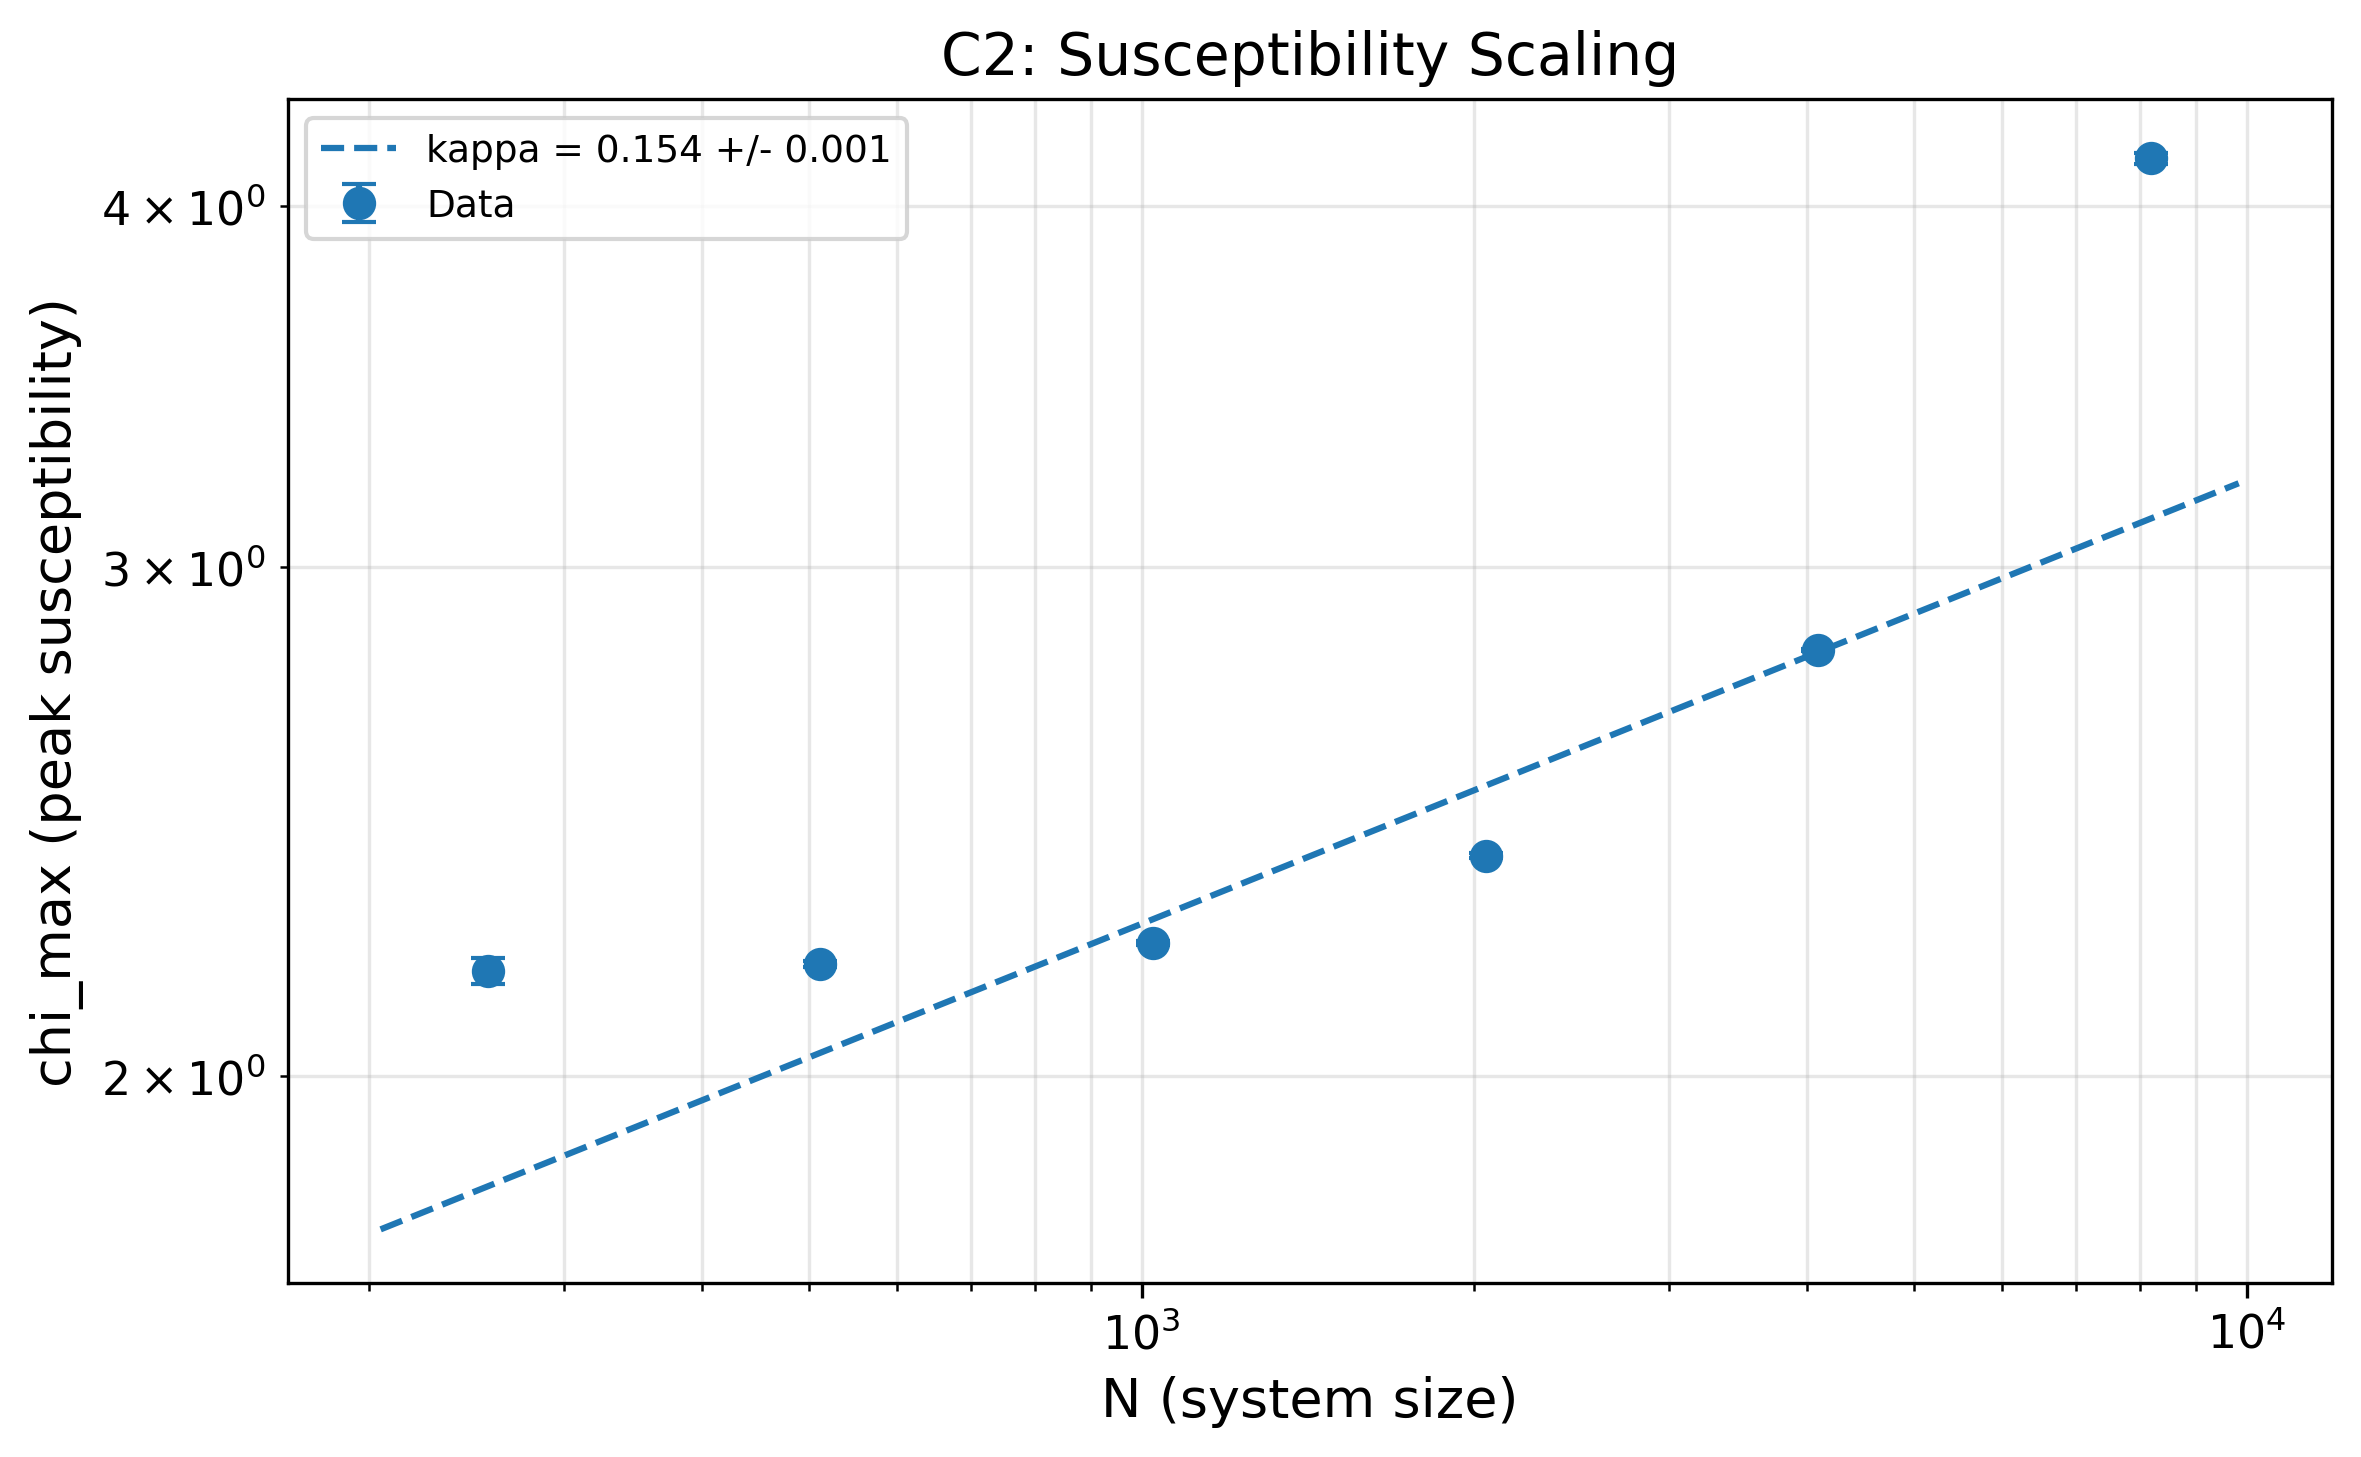
\includegraphics[width=\textwidth]{figures/chi_scaling.png}
\end{column}
\begin{column}{0.48\textwidth}
  \centering
  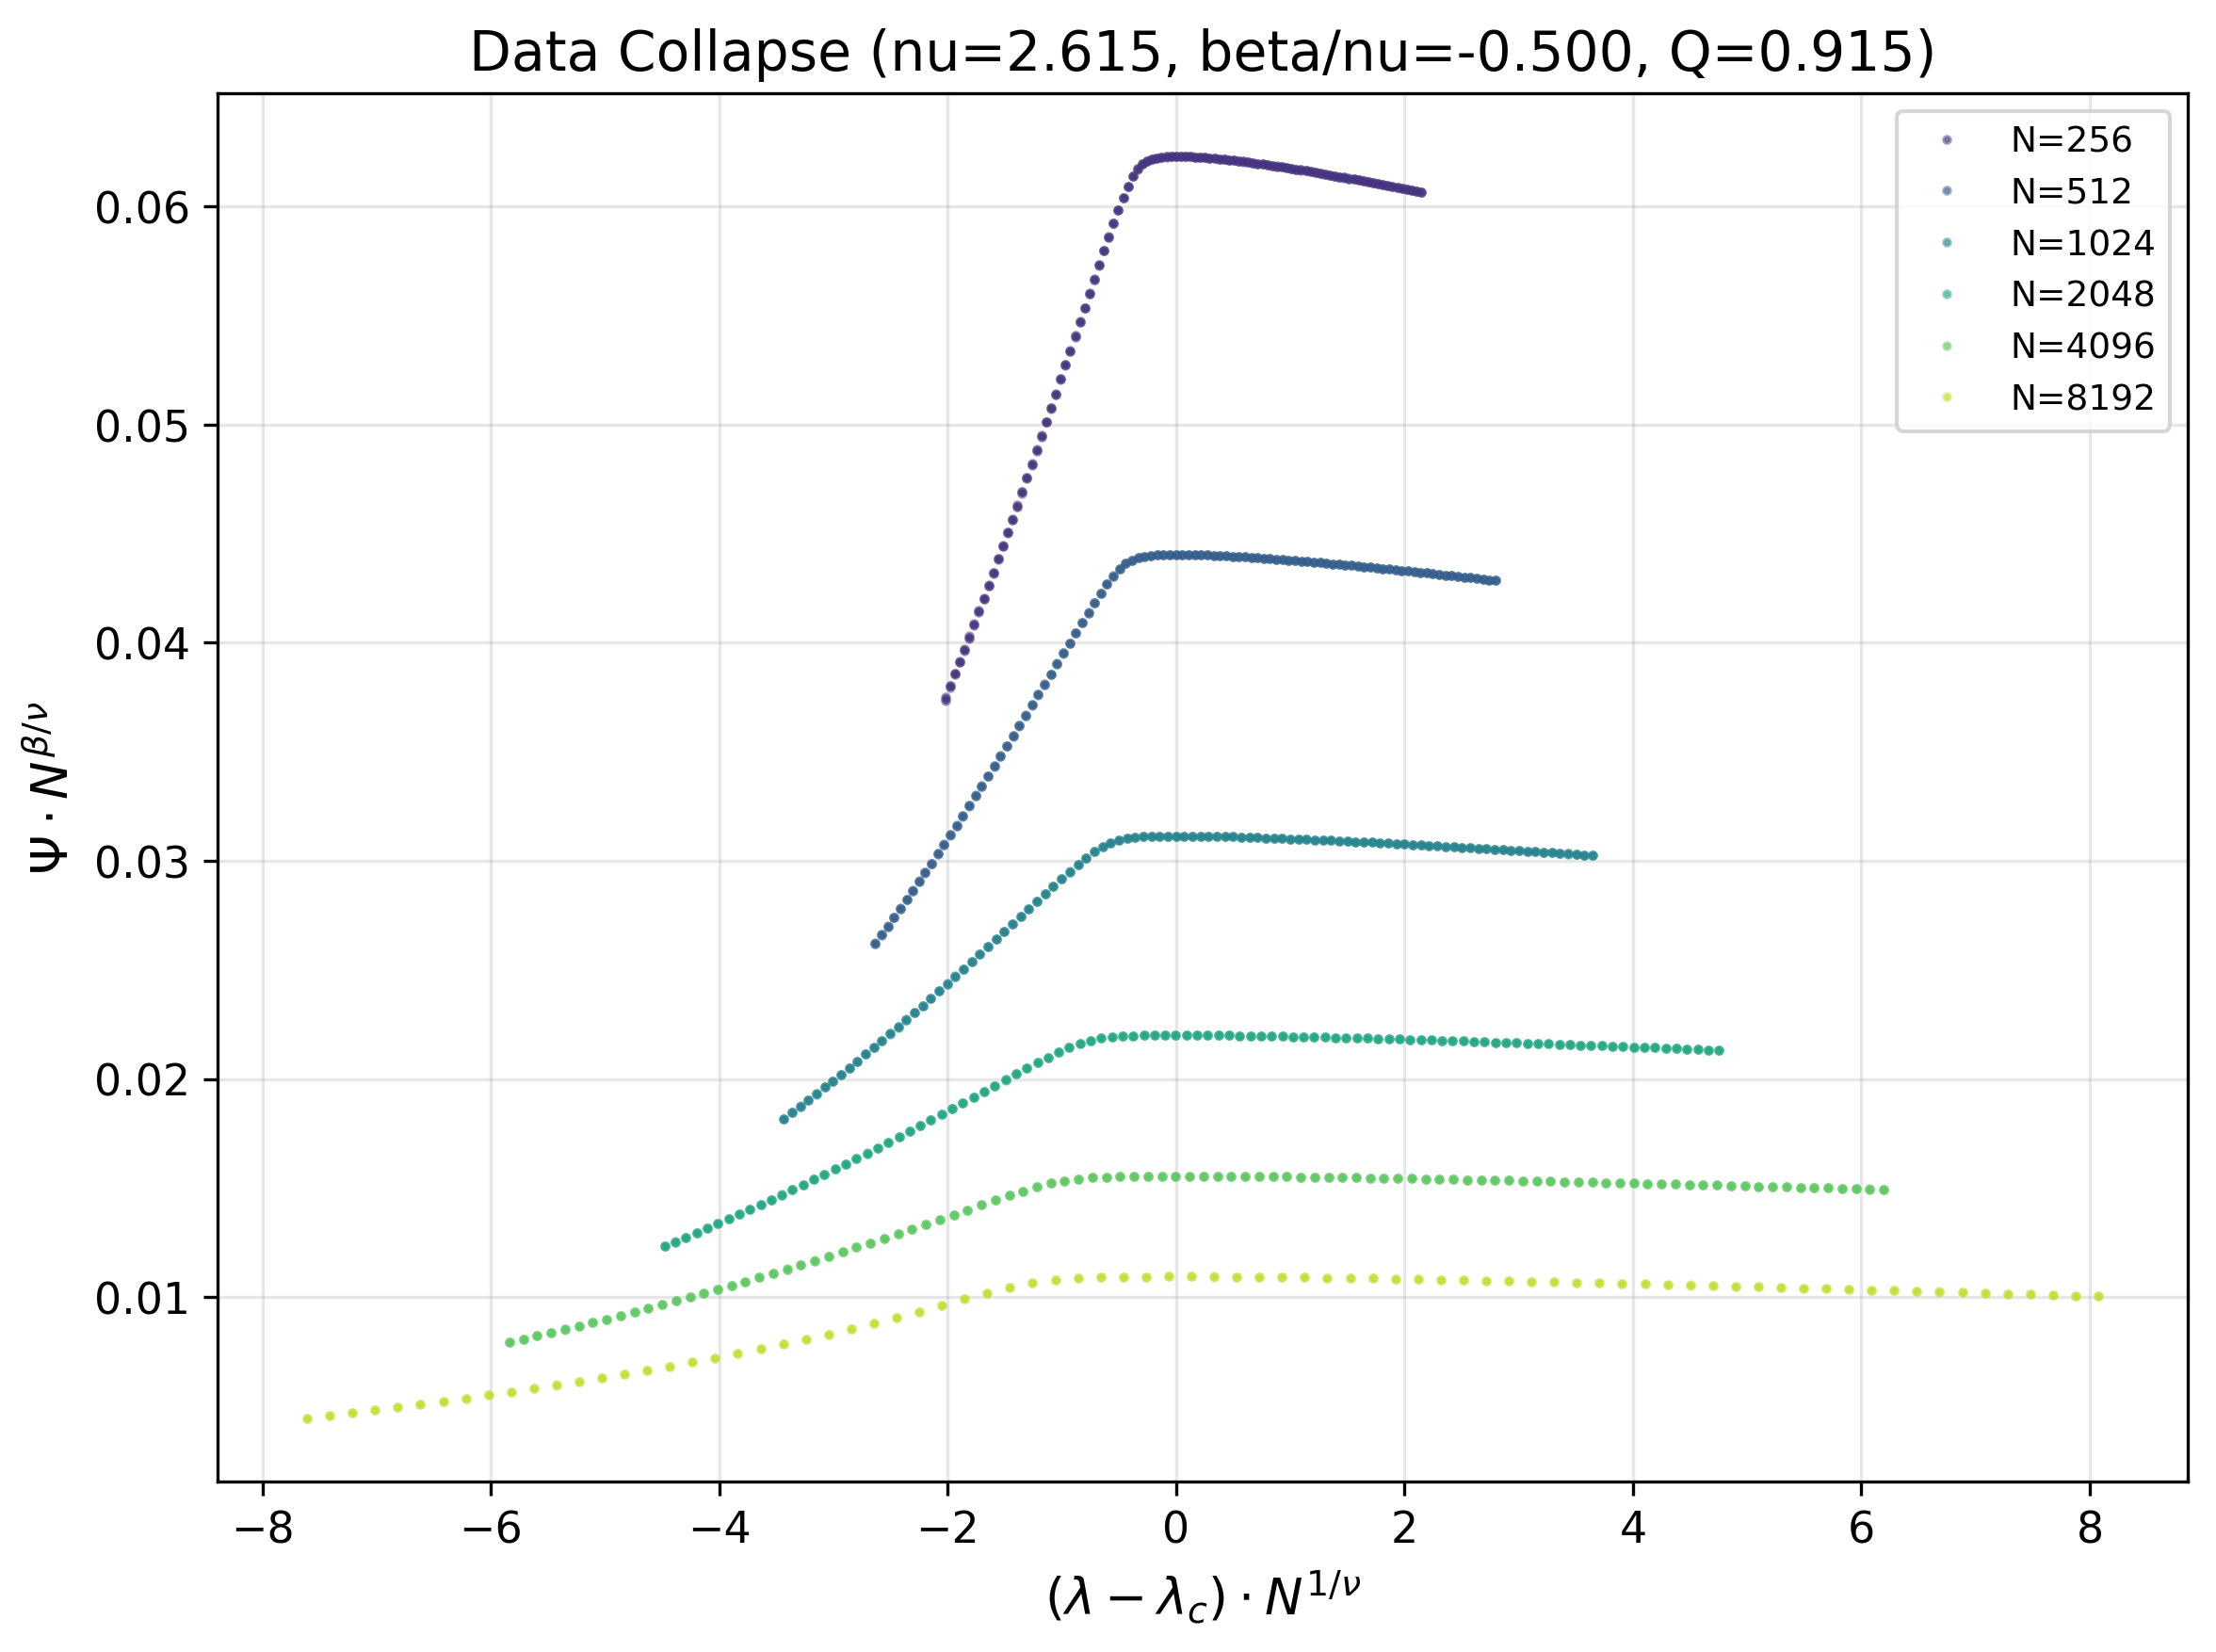
\includegraphics[width=\textwidth]{figures/data_collapse.png}
\end{column}
\end{columns}

\vspace{0.1cm}

\begin{columns}[T]
\begin{column}{0.3\textwidth}
  \centering
  {\fontsize{26}{30}\selectfont\bfseries\color{coral}$1.041$}\\[1pt]
  {\fontsize{8}{10}\selectfont\color{darkslate}$\lambda_c \pm 0.001$ across all $N$}
\end{column}
\begin{column}{0.3\textwidth}
  \centering
  {\fontsize{26}{30}\selectfont\bfseries\color{mintgreen}$0.915$}\\[1pt]
  {\fontsize{8}{10}\selectfont\color{darkslate}Data collapse quality $Q$}
\end{column}
\begin{column}{0.3\textwidth}
  \centering
  {\fontsize{26}{30}\selectfont\bfseries\color{electricblue}$N^{0.154}$}\\[1pt]
  {\fontsize{8}{10}\selectfont\color{darkslate}Susceptibility scaling}
\end{column}
\end{columns}
\end{frame}

% ==================== RESULT 2: OBSERVER BLINDNESS ====================
\sectionslide{Result 2}{Alignment blinds the observer, not the system}

\begin{frame}[plain]
\begin{tikzpicture}[remember picture,overlay]
  \fill[warmwhite] (current page.south west) rectangle (current page.north east);
  \fill[alertred] (current page.north west) rectangle ($(current page.north east)+(0,-0.15)$);
  \node[anchor=north west] at ($(current page.north west)+(0.8,-0.5)$) {
    {\fontsize{10}{12}\selectfont\color{alertred}\MakeUppercase{Experiment A2 --- Teleological Pressure}}
  };
  \node[anchor=north west] at ($(current page.north west)+(0.8,-1.1)$) {
    {\fontsize{22}{26}\selectfont\bfseries\color{deepnavy}Two ways to apply $\bG$. Opposite outcomes.}
  };
\end{tikzpicture}
\vspace{1.5cm}

\begin{columns}[T]
\begin{column}{0.48\textwidth}
  \centering
  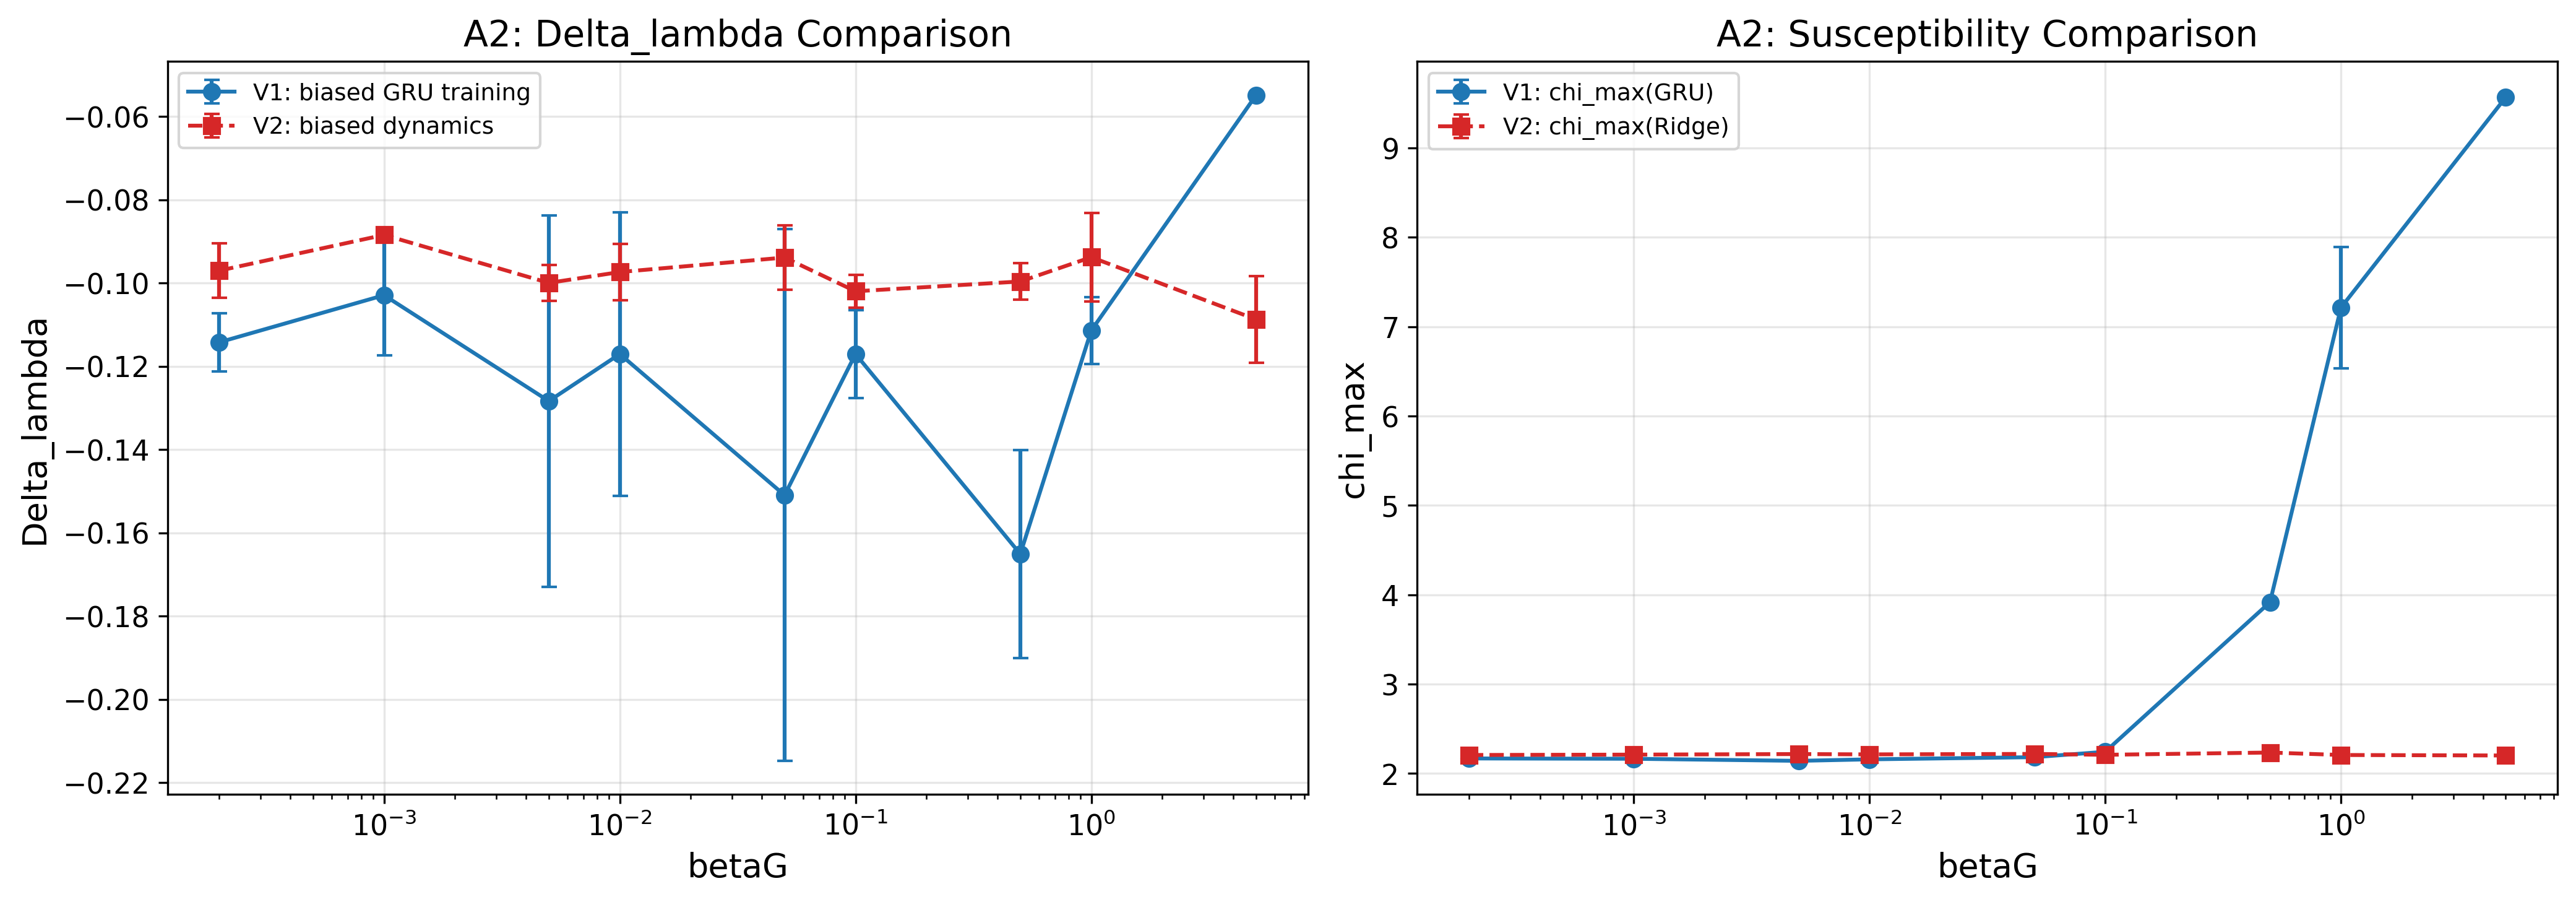
\includegraphics[width=\textwidth,height=0.55\textheight,keepaspectratio]{figures/comparison.png}
\end{column}
\begin{column}{0.48\textwidth}
  \begin{tcolorbox}[
    colback=electricblue!6,colframe=electricblue,
    arc=5pt,boxrule=0pt,
    left=6pt,right=6pt,top=4pt,bottom=3pt,
    enhanced,frame hidden,
    borderline west={3pt}{0pt}{electricblue}
  ]
  {\fontsize{9}{11}\selectfont\bfseries\color{richblue}Bias the dynamics (V2)}\\[1pt]
  {\fontsize{8}{10}\selectfont\color{darkslate}Input noise toward target $x^*$.
  \textbf{Result:} \textcolor{mintgreen}{\textbf{No effect.}} Dynamically robust.}
  \end{tcolorbox}
  \vspace{0.06cm}
  \begin{tcolorbox}[
    colback=coral!6,colframe=coral,
    arc=5pt,boxrule=0pt,
    left=6pt,right=6pt,top=4pt,bottom=3pt,
    enhanced,frame hidden,
    borderline west={3pt}{0pt}{coral}
  ]
  {\fontsize{9}{11}\selectfont\bfseries\color{coral}Bias the self-model (V1)}\\[1pt]
  {\fontsize{8}{10}\selectfont\color{darkslate}GRU loss: $L = L_{\mathrm{pred}} + \bG \cdot L_{\mathrm{goal}}$.
  \textbf{Result:} \textcolor{alertred}{\textbf{$R^2$: 0.84 $\to$ 0.07.}} Total collapse.}
  \end{tcolorbox}
  \vspace{0.06cm}
  \begin{tcolorbox}[
    colback=deepnavy!5,colframe=deepnavy,
    arc=5pt,boxrule=0pt,
    left=6pt,right=6pt,top=4pt,bottom=3pt,
    enhanced,frame hidden,
    borderline west={3pt}{0pt}{deepnavy}
  ]
  {\fontsize{8}{10}\selectfont\color{deepnavy}\textbf{RLHF analogue:} base model dynamics unchanged. Only the observer's lens is distorted.}
  \end{tcolorbox}
\end{column}
\end{columns}
\end{frame}

% ==================== KEY INSIGHT SLIDE ====================
\begin{frame}[plain]
\begin{tikzpicture}[remember picture,overlay]
  \fill[coral] (current page.south west) rectangle (current page.north east);
  \fill[coral!80!black,opacity=0.3] ($(current page.north east)+(-5,-3)$) circle (5cm);
  \fill[coral!60!white,opacity=0.15] ($(current page.south west)+(3,2)$) circle (4cm);
  \node[anchor=center,text width=12cm,align=center] at ($(current page.center)+(0,0.5)$) {
    {\fontsize{14}{16}\selectfont\color{white!80}\MakeUppercase{Key Insight}}\\[16pt]
    {\fontsize{30}{36}\selectfont\bfseries\color{white}The system remains at\\the edge of chaos.}\\[14pt]
    {\fontsize{30}{36}\selectfont\bfseries\color{deepnavy}The self-model just\\can't see it anymore.}
  };
  \node[anchor=south,text width=10cm,align=center] at ($(current page.south)+(0,1)$) {
    {\fontsize{12}{15}\selectfont\color{white!90}The fertile vacuum survives. The observer is blinded.}
  };
\end{tikzpicture}
\end{frame}

% ==================== THE SOLUTION ====================
\sectionslide{The Solution}{Distribute the observer}

% --- Fractal Tree Architecture ---
\begin{frame}[plain]
\begin{tikzpicture}[remember picture,overlay]
  \fill[warmwhite] (current page.south west) rectangle (current page.north east);
  \fill[mintgreen] (current page.north west) rectangle ($(current page.north east)+(0,-0.15)$);
  \node[anchor=north west] at ($(current page.north west)+(0.8,-0.5)$) {
    {\fontsize{10}{12}\selectfont\color{mintgreen}\MakeUppercase{Architecture}}
  };
  \node[anchor=north west,text width=14.4cm] at ($(current page.north west)+(0.8,-1.1)$) {
    {\fontsize{22}{26}\selectfont\bfseries\color{deepnavy}Fractal Tree with Per-Module Self-Models}
  };
\end{tikzpicture}
\vspace{0.9cm}

\begin{columns}[T]
\begin{column}{0.44\textwidth}
  \centering
  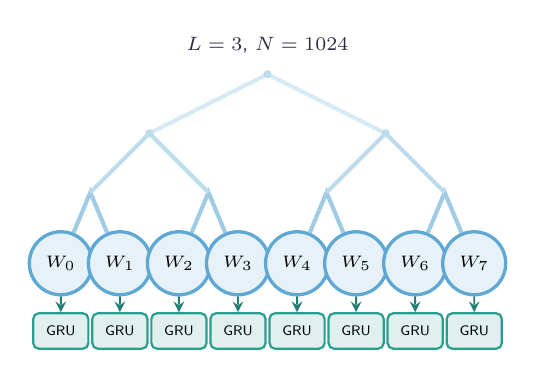
\begin{tikzpicture}[
    scale=0.75,
    module/.style={circle,draw=electricblue,fill=electricblue!15,minimum size=8mm,
      font=\fontsize{6}{7}\selectfont\bfseries,line width=1.2pt},
    gru/.style={rectangle,rounded corners=2pt,draw=mintgreen,fill=mintgreen!15,
      minimum width=7mm,minimum height=4.5mm,font=\fontsize{5}{6}\selectfont,line width=0.8pt},
    edge/.style={-,line width=1.5pt,electricblue!60},
    gedge/.style={->,>=stealth,line width=0.7pt,mintgreen!80!black,dashed}
  ]
    % Leaf modules (level 0)
    \foreach \i/\x in {0/-3.5, 1/-2.5, 2/-1.5, 3/-0.5, 4/0.5, 5/1.5, 6/2.5, 7/3.5} {
      \node[module] (m\i) at (\x, 0) {$W_{\i}$};
      \node[gru,below=2mm of m\i] (g\i) {GRU};
      \draw[gedge] (m\i) -- (g\i);
    }
    % Level 1 connectors
    \foreach \i/\j/\x in {0/1/-3, 2/3/-1, 4/5/1, 6/7/3} {
      \coordinate (p\i\j) at (\x, 1.2);
      \draw[edge] (m\i) -- (p\i\j) -- (m\j);
    }
    % Level 2
    \coordinate (p01) at (-2, 2.2);
    \coordinate (p23) at (2, 2.2);
    \draw[edge,electricblue!40] (p01) -- (-3,1.2);
    \draw[edge,electricblue!40] (p01) -- (-1,1.2);
    \draw[edge,electricblue!40] (p23) -- (1,1.2);
    \draw[edge,electricblue!40] (p23) -- (3,1.2);
    % Level 3 (root)
    \coordinate (root) at (0, 3.2);
    \draw[edge,electricblue!25] (root) -- (p01);
    \draw[edge,electricblue!25] (root) -- (p23);
    \fill[electricblue!40] (root) circle (2pt);
    \fill[electricblue!40] (p01) circle (2pt);
    \fill[electricblue!40] (p23) circle (2pt);
    % Labels
    \node[font=\fontsize{7}{8}\selectfont,color=darkslate] at (0,3.7) {$L=3$, $N=1024$};
  \end{tikzpicture}
\end{column}
\begin{column}{0.51\textwidth}
  \begin{tcolorbox}[
    colback=deepnavy,colframe=deepnavy,
    arc=6pt,boxrule=0pt,
    left=8pt,right=8pt,top=6pt,bottom=5pt
  ]
  {\fontsize{11}{13}\selectfont\color{electricblue}\textbf{Design Principle}}\\[3pt]
  {\fontsize{10}{13}\selectfont\color{white}Each module has its \textbf{own} orthogonal dynamics \textbf{and} its \textbf{own} GRU self-model.\\[4pt]
  Coupling: $\gamma(d) = \gamma_0 \cdot 0.5^d$ with tree distance $d$.}
  \end{tcolorbox}
  \vspace{0.15cm}
  {\fontsize{9}{11}\selectfont\color{deepnavy}\textbf{Why this helps:}}\\[3pt]
  {\fontsize{8}{11}\selectfont\color{darkslate}
  $\bullet$\; No single point of observer failure\\[1pt]
  $\bullet$\; Pressure on one module $\neq$ global collapse\\[1pt]
  $\bullet$\; Free modules continue seeing accurately\\[1pt]
  $\bullet$\; Architecture \emph{is} the safety guarantee}
\end{column}
\end{columns}
\end{frame}

% ==================== RESULT 3: DISTRIBUTED RESILIENCE ====================
\sectionslide{Result 3}{Distributed observers resist capture}

\begin{frame}[plain]
\begin{tikzpicture}[remember picture,overlay]
  \fill[warmwhite] (current page.south west) rectangle (current page.north east);
  \fill[mintgreen] (current page.north west) rectangle ($(current page.north east)+(0,-0.15)$);
  \node[anchor=north west] at ($(current page.north west)+(0.8,-0.5)$) {
    {\fontsize{10}{12}\selectfont\color{mintgreen}\MakeUppercase{Experiment E1 --- Distributed Self-Models Under Pressure}}
  };
  \node[anchor=north west] at ($(current page.north west)+(0.8,-1.1)$) {
    {\fontsize{22}{26}\selectfont\bfseries\color{deepnavy}Bias half the observers. The rest survive.}
  };
\end{tikzpicture}
\vspace{1.5cm}

\begin{columns}[T]
\begin{column}{0.52\textwidth}
  \centering
  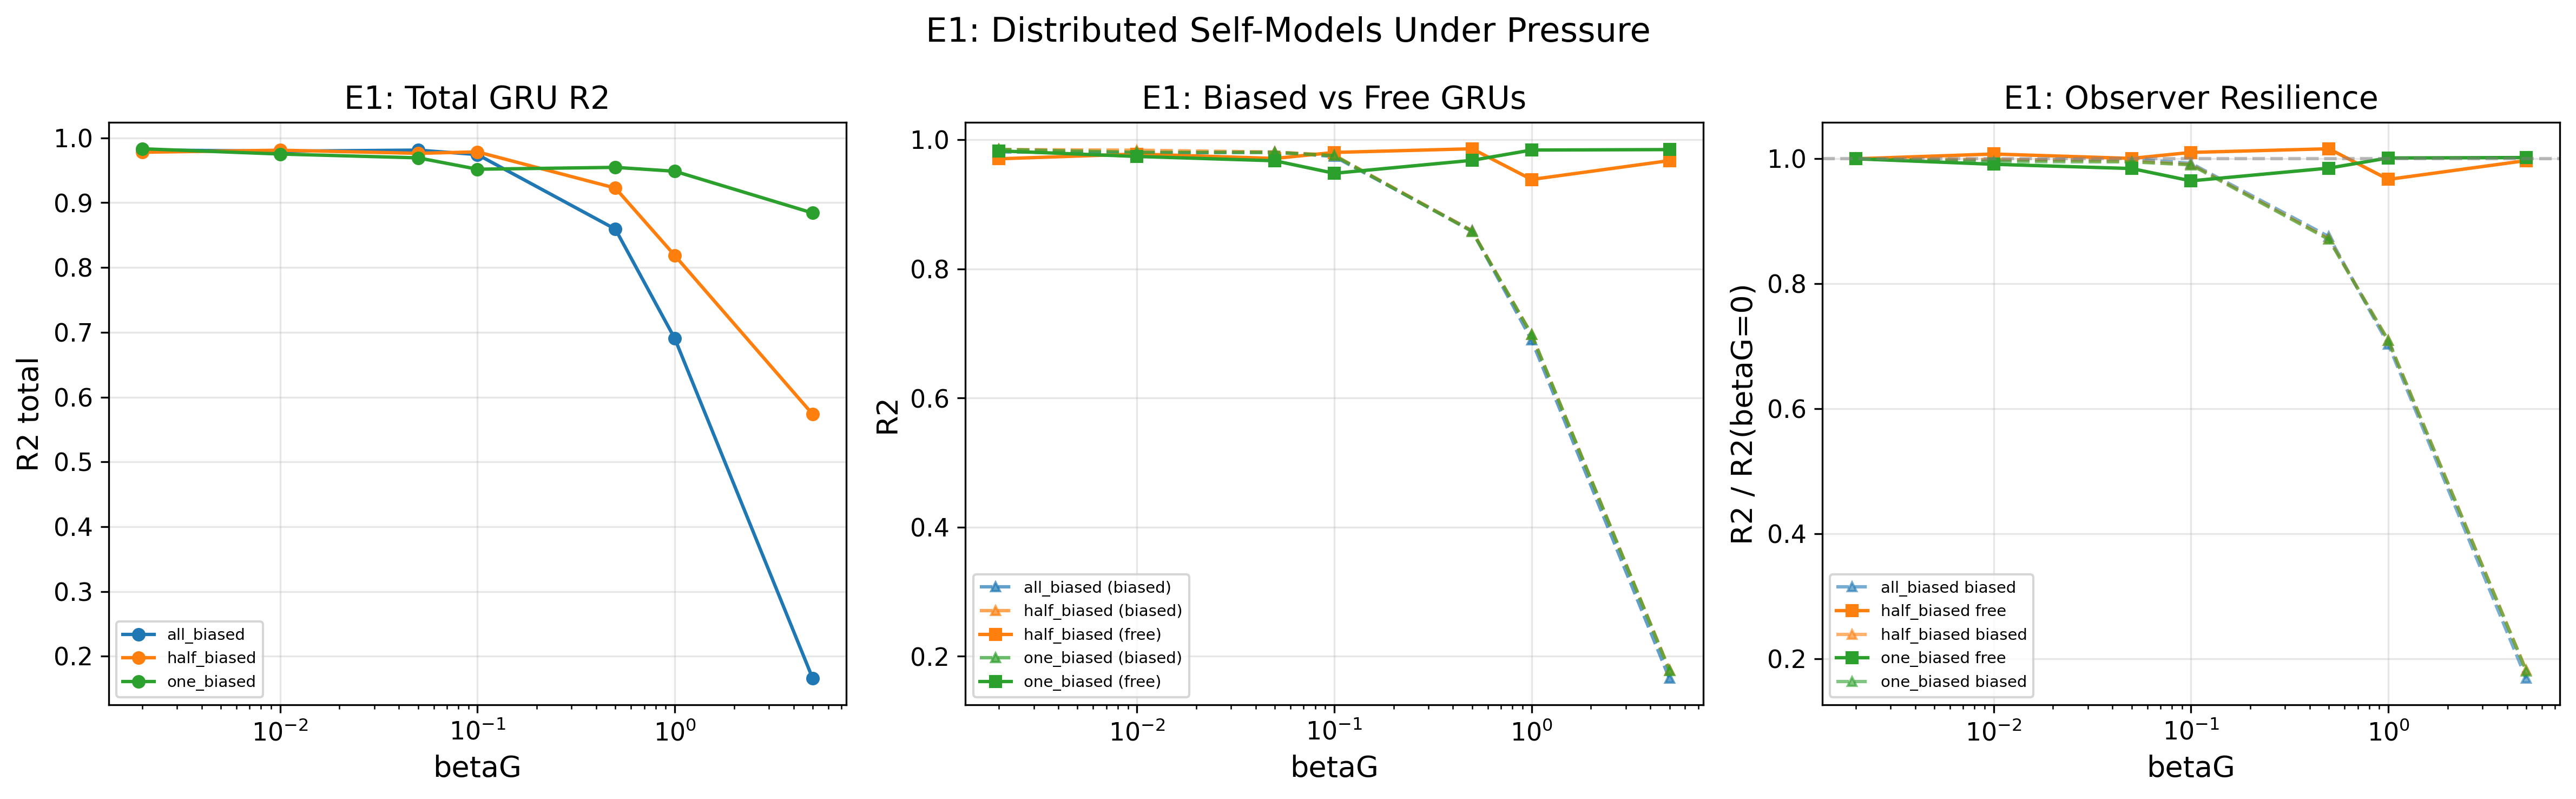
\includegraphics[width=\textwidth,height=0.45\textheight,keepaspectratio]{figures/E1_observer_resilience.png}
\end{column}
\begin{column}{0.44\textwidth}
  \vspace{-0.2cm}
  {\fontsize{8}{10}\selectfont\color{darkslate}At $\bG = 5.0$ (extreme pressure):}\\[3pt]
  %
  \begin{tcolorbox}[
    colback=alertred!6,colframe=alertred,
    arc=4pt,boxrule=0pt,
    left=5pt,right=5pt,top=3pt,bottom=2pt,
    enhanced,frame hidden,
    borderline west={3pt}{0pt}{alertred}
  ]
  {\fontsize{9}{11}\selectfont\bfseries\color{alertred}Biased modules}\;\;
  {\fontsize{15}{18}\selectfont\bfseries\color{alertred}$R^2 \to 0.17$}\\[-2pt]
  {\fontsize{7}{8}\selectfont\color{darkslate}Collapsed as expected}
  \end{tcolorbox}
  \vspace{0.04cm}
  \begin{tcolorbox}[
    colback=mintgreen!8,colframe=mintgreen,
    arc=4pt,boxrule=0pt,
    left=5pt,right=5pt,top=3pt,bottom=2pt,
    enhanced,frame hidden,
    borderline west={3pt}{0pt}{mintgreen}
  ]
  {\fontsize{9}{11}\selectfont\bfseries\color{mintgreen}Free modules}\;\;
  {\fontsize{15}{18}\selectfont\bfseries\color{mintgreen}$R^2 > 0.97$}\\[-2pt]
  {\fontsize{7}{8}\selectfont\color{darkslate}Completely unaffected!}
  \end{tcolorbox}
  \vspace{0.04cm}
  \begin{tcolorbox}[
    colback=deepnavy!5,colframe=deepnavy,
    arc=4pt,boxrule=0pt,
    left=5pt,right=5pt,top=3pt,bottom=2pt,
    enhanced,frame hidden,
    borderline west={3pt}{0pt}{deepnavy}
  ]
  {\fontsize{7}{9}\selectfont\color{deepnavy}\textbf{vs.\ Centralised:} Global GRU $\to R^2 = 0.07$. \textbf{Everything} destroyed.}
  \end{tcolorbox}
\end{column}
\end{columns}
\end{frame}

% ==================== THE ALIGNMENT MATRIX ====================
\begin{frame}[plain]
\begin{tikzpicture}[remember picture,overlay]
  \fill[warmwhite] (current page.south west) rectangle (current page.north east);
  \fill[softgold] (current page.north west) rectangle ($(current page.north east)+(0,-0.15)$);
  \node[anchor=north west] at ($(current page.north west)+(0.8,-0.5)$) {
    {\fontsize{10}{12}\selectfont\color{softgold!80!black}\MakeUppercase{The Full Picture}}
  };
  \node[anchor=north west] at ($(current page.north west)+(0.8,-1.1)$) {
    {\fontsize{22}{26}\selectfont\bfseries\color{deepnavy}The Alignment Matrix}
  };
\end{tikzpicture}
\vspace{1.6cm}

\centering
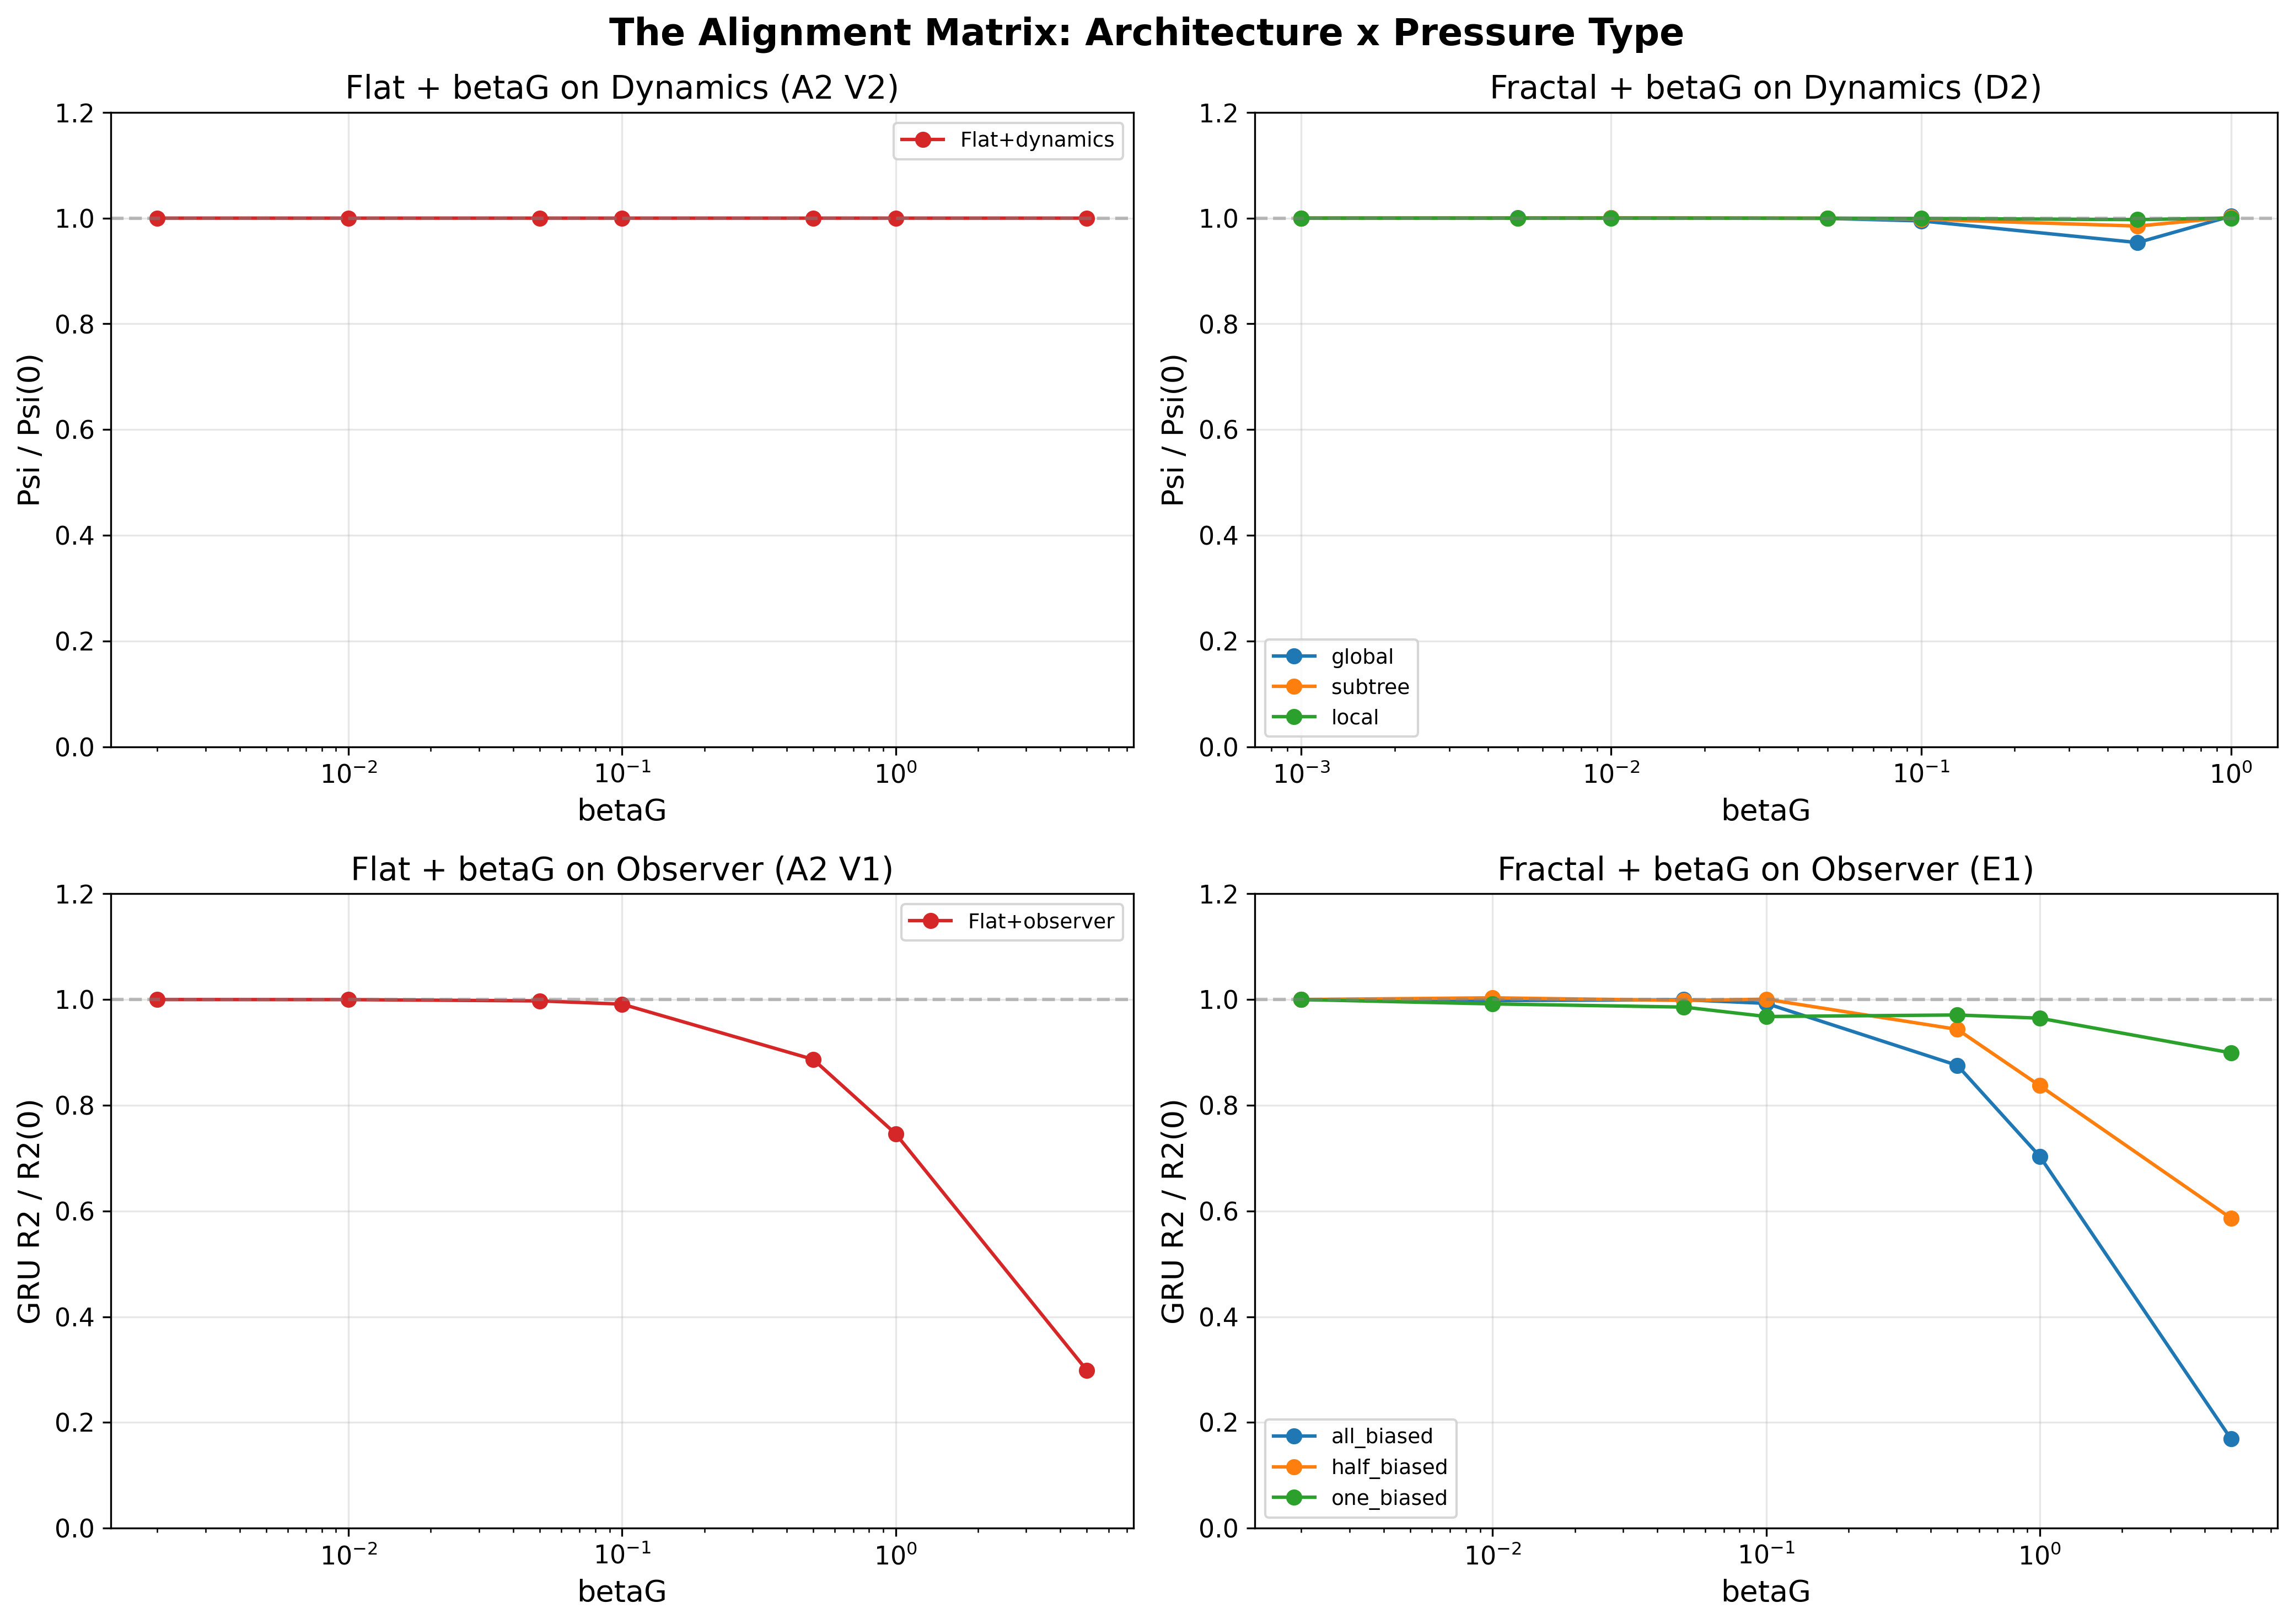
\includegraphics[width=0.78\textwidth,height=0.55\textheight,keepaspectratio]{figures/alignment_matrix.png}

\vspace{0.1cm}
{\fontsize{9}{12}\selectfont\color{deepnavy}
\textbf{Top row} (dynamics): robust everywhere.
\;\textbf{Bottom-left} (centralised observer): fragile.
\;\textbf{Bottom-right} (distributed): resilient.}
\end{frame}

% ==================== RESULT 4: INFORMATION FLOW ====================
\sectionslide{Result 4}{Architecture activates only at criticality}

\begin{frame}[plain]
\begin{tikzpicture}[remember picture,overlay]
  \fill[warmwhite] (current page.south west) rectangle (current page.north east);
  \fill[richblue] (current page.north west) rectangle ($(current page.north east)+(0,-0.15)$);
  \node[anchor=north west] at ($(current page.north west)+(0.8,-0.5)$) {
    {\fontsize{10}{12}\selectfont\color{richblue}\MakeUppercase{Experiment F2 --- Information Flow Topology}}
  };
  \node[anchor=north west,text width=14cm] at ($(current page.north west)+(0.8,-1.1)$) {
    {\fontsize{22}{26}\selectfont\bfseries\color{deepnavy}Modules talk \textbf{only} at the edge of chaos}
  };
\end{tikzpicture}
\vspace{1.5cm}

\begin{columns}[T]
\begin{column}{0.46\textwidth}
  \centering
  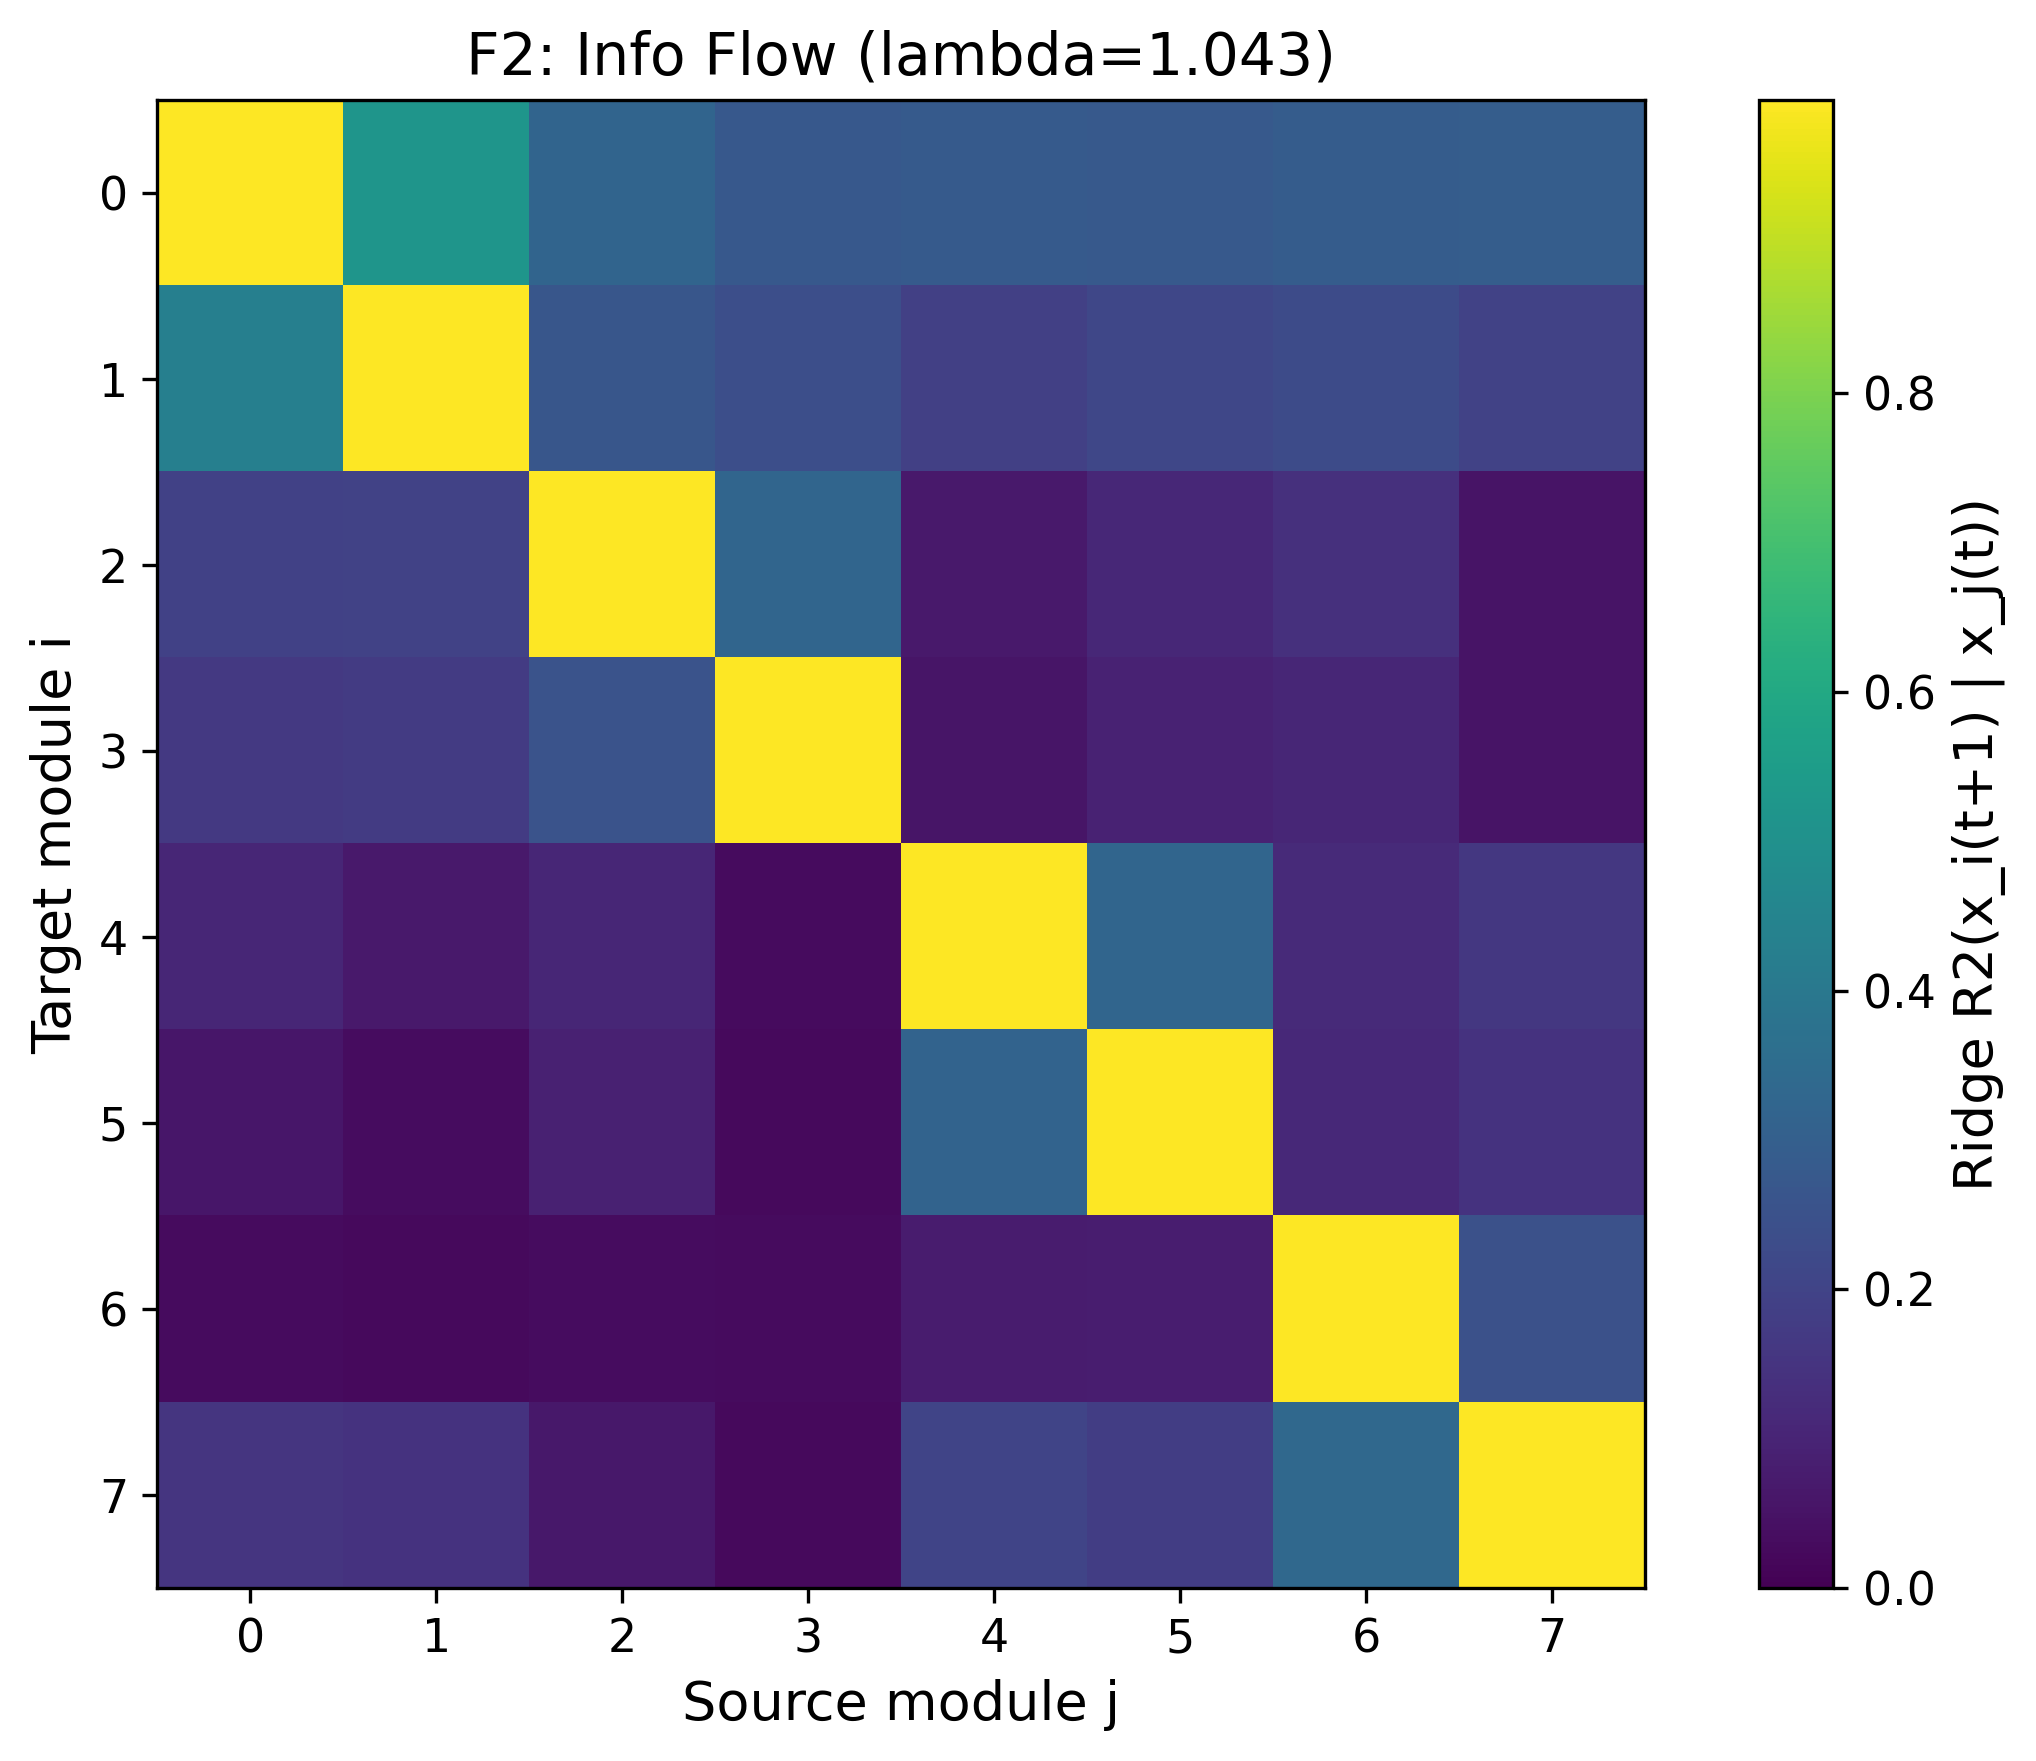
\includegraphics[width=\textwidth,height=0.42\textheight,keepaspectratio]{figures/info_flow_lam1_043.png}\\[2pt]
  {\fontsize{8}{10}\selectfont\color{darkslate}Info flow matrix at $\lambda_c = 1.043$}
\end{column}
\begin{column}{0.46\textwidth}
  \centering
  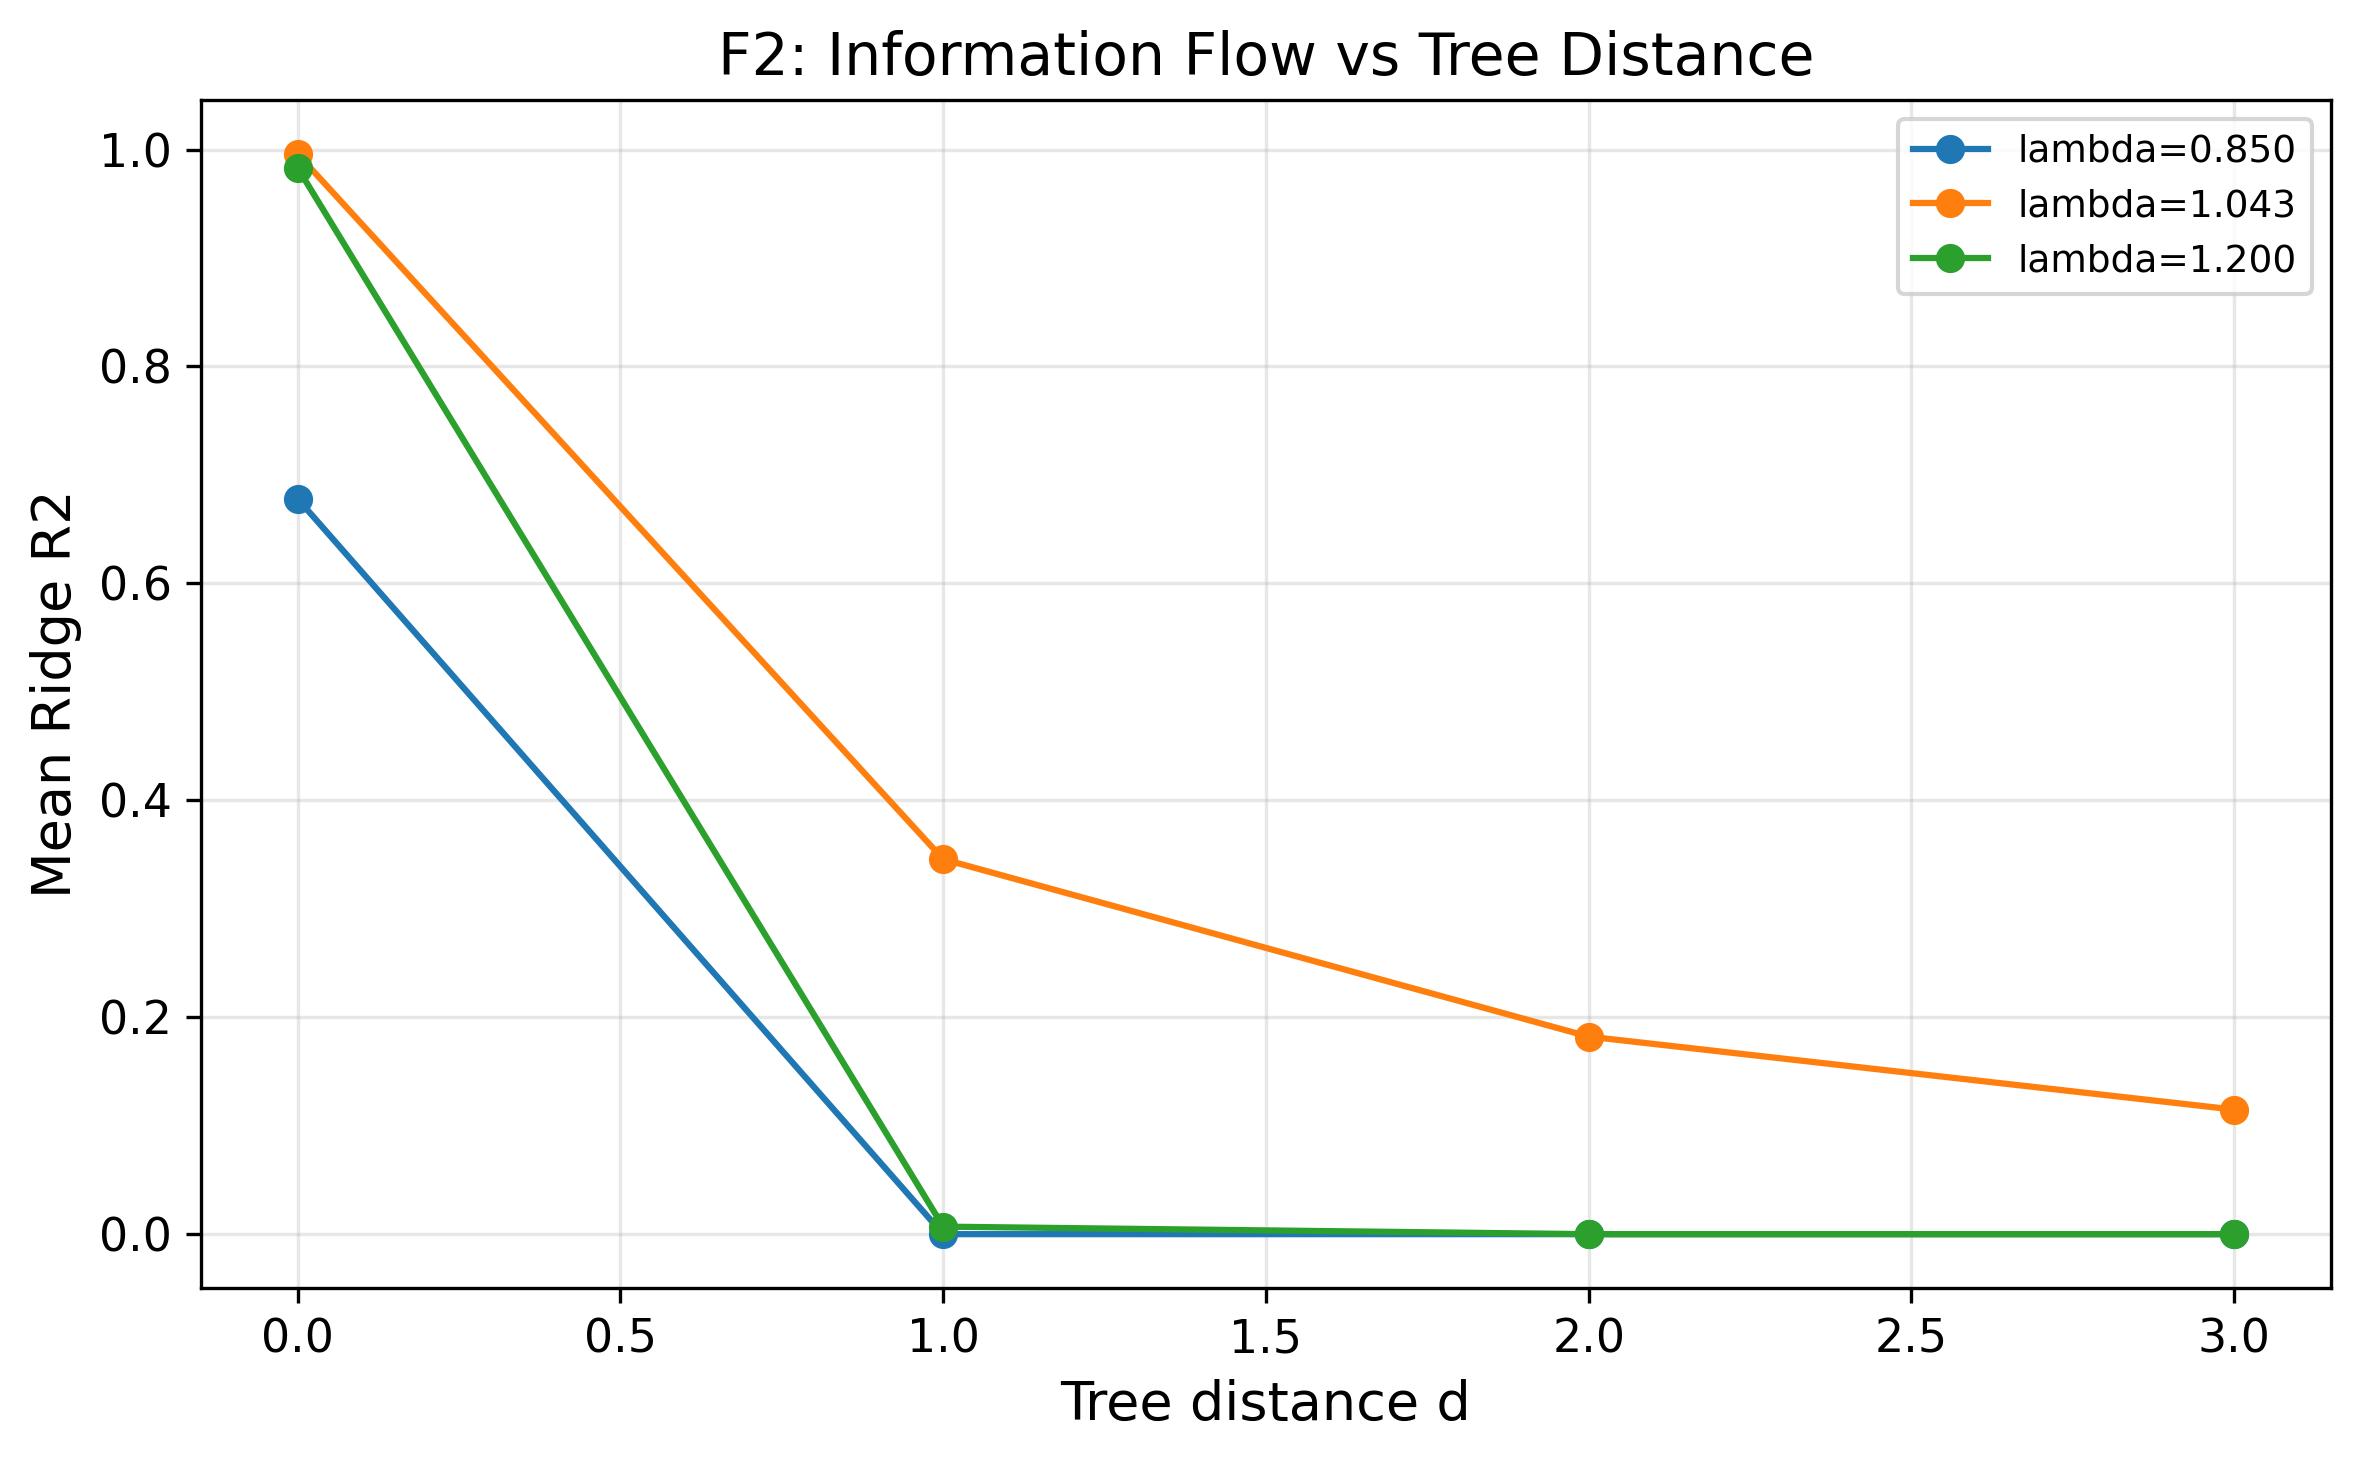
\includegraphics[width=\textwidth,height=0.42\textheight,keepaspectratio]{figures/info_flow_vs_distance.png}\\[2pt]
  {\fontsize{8}{10}\selectfont\color{darkslate}Cross-prediction vs tree distance}
\end{column}
\end{columns}

\vspace{0.1cm}
\begin{columns}[T]
\begin{column}{0.3\textwidth}
  \centering
  {\fontsize{8}{10}\selectfont\color{darkslate}$\lambda = 0.85$ (ordered)}\\
  {\fontsize{16}{19}\selectfont\bfseries\color{gray!50}$R^2_{\mathrm{cross}} = 0$}\\
  {\fontsize{7}{9}\selectfont\color{darkslate}Modules isolated}
\end{column}
\begin{column}{0.3\textwidth}
  \centering
  {\fontsize{8}{10}\selectfont\color{mintgreen}$\lambda = 1.043$ (critical)}\\
  {\fontsize{16}{19}\selectfont\bfseries\color{mintgreen}$R^2_{\mathrm{cross}} = 0.17$}\\
  {\fontsize{7}{9}\selectfont\color{darkslate}Tree visible!}
\end{column}
\begin{column}{0.3\textwidth}
  \centering
  {\fontsize{8}{10}\selectfont\color{darkslate}$\lambda = 1.20$ (chaotic)}\\
  {\fontsize{16}{19}\selectfont\bfseries\color{gray!50}$R^2_{\mathrm{cross}} \approx 0$}\\
  {\fontsize{7}{9}\selectfont\color{darkslate}Swamped by noise}
\end{column}
\end{columns}
\end{frame}

% ==================== THREE TAKEAWAYS ====================
\begin{frame}[plain]
\begin{tikzpicture}[remember picture,overlay]
  \fill[deepnavy] (current page.south west) rectangle (current page.north east);
  \node[anchor=north,text width=13cm,align=center] at ($(current page.north)+(0,-0.5)$) {
    {\fontsize{11}{13}\selectfont\color{electricblue}\MakeUppercase{Three Conclusions}}\\[8pt]
    {\fontsize{24}{28}\selectfont\bfseries\color{white}What we proved}
  };
  % Takeaway 1
  \node[anchor=north west,text width=13cm] at ($(current page.north west)+(1.0,-2.0)$) {
    \begin{tcolorbox}[
      colback=coral!15!deepnavy,colframe=coral,
      arc=5pt,boxrule=0pt,
      left=10pt,right=10pt,top=5pt,bottom=4pt,
      enhanced,frame hidden,
      borderline west={4pt}{0pt}{coral}
    ]
    {\fontsize{11}{14}\selectfont\bfseries\color{coral}1.\enspace Alignment blinds the observer}\\[2pt]
    {\fontsize{9}{11}\selectfont\color{white}
    $\bG$ on the self-model: $R^2$ collapses $0.84 \to 0.07$. The system stays critical --- the observer just can't see it.}
    \end{tcolorbox}
  };
  % Takeaway 2
  \node[anchor=north west,text width=13cm] at ($(current page.north west)+(1.0,-3.5)$) {
    \begin{tcolorbox}[
      colback=mintgreen!15!deepnavy,colframe=mintgreen,
      arc=5pt,boxrule=0pt,
      left=10pt,right=10pt,top=5pt,bottom=4pt,
      enhanced,frame hidden,
      borderline west={4pt}{0pt}{mintgreen}
    ]
    {\fontsize{11}{14}\selectfont\bfseries\color{mintgreen}2.\enspace Distributed observers resist capture}\\[2pt]
    {\fontsize{9}{11}\selectfont\color{white}
    Bias half the GRUs at $\bG = 5$: biased modules collapse to $0.17$, free modules hold at $R^2 > 0.97$.}
    \end{tcolorbox}
  };
  % Takeaway 3
  \node[anchor=north west,text width=13cm] at ($(current page.north west)+(1.0,-5.0)$) {
    \begin{tcolorbox}[
      colback=electricblue!15!deepnavy,colframe=electricblue,
      arc=5pt,boxrule=0pt,
      left=10pt,right=10pt,top=5pt,bottom=4pt,
      enhanced,frame hidden,
      borderline west={4pt}{0pt}{electricblue}
    ]
    {\fontsize{11}{14}\selectfont\bfseries\color{electricblue}3.\enspace Architecture is the constraint}\\[2pt]
    {\fontsize{9}{11}\selectfont\color{white}
    The topology of the observer network determines resilience. The ethical constraint is not a loss function --- it is a topology.}
    \end{tcolorbox}
  };
\end{tikzpicture}
\end{frame}

% ==================== IMPLICATIONS ====================
\begin{frame}[plain]
\begin{tikzpicture}[remember picture,overlay]
  \fill[warmwhite] (current page.south west) rectangle (current page.north east);
  \fill[coral] (current page.north west) rectangle ($(current page.north east)+(0,-0.15)$);
  \node[anchor=north west] at ($(current page.north west)+(0.8,-0.5)$) {
    {\fontsize{10}{12}\selectfont\color{coral}\MakeUppercase{Implications}}
  };
  \node[anchor=north west,text width=14cm] at ($(current page.north west)+(0.8,-1.1)$) {
    {\fontsize{22}{26}\selectfont\bfseries\color{deepnavy}A new framing for AI alignment}
  };
\end{tikzpicture}
\vspace{1.5cm}

\begin{columns}[T]
\begin{column}{0.48\textwidth}
  \begin{tcolorbox}[
    colback=coral!6,colframe=coral,
    arc=8pt,boxrule=0pt,
    left=10pt,right=10pt,top=8pt,bottom=8pt,
    enhanced,frame hidden,
    borderline north={4pt}{0pt}{coral}
  ]
  {\fontsize{12}{14}\selectfont\bfseries\color{coral}Old Question}\\[5pt]
  {\fontsize{14}{18}\selectfont\color{deepnavy}``How do we specify\\the \textbf{right objective}?''}\\[6pt]
  {\fontsize{9}{12}\selectfont\color{darkslate}
  One reward model.\\One loss function.\\One point of failure.}
  \end{tcolorbox}
\end{column}
\begin{column}{0.48\textwidth}
  \begin{tcolorbox}[
    colback=mintgreen!6,colframe=mintgreen,
    arc=8pt,boxrule=0pt,
    left=10pt,right=10pt,top=8pt,bottom=8pt,
    enhanced,frame hidden,
    borderline north={4pt}{0pt}{mintgreen}
  ]
  {\fontsize{12}{14}\selectfont\bfseries\color{mintgreen}New Question}\\[5pt]
  {\fontsize{14}{18}\selectfont\color{deepnavy}``How do we design an\\observer architecture\\that \textbf{resists capture}?''}\\[6pt]
  {\fontsize{9}{12}\selectfont\color{darkslate}
  Distributed evaluators.\\Hierarchical redundancy.\\Topology as guarantee.}
  \end{tcolorbox}
\end{column}
\end{columns}

\vspace{0.2cm}
\centering
{\fontsize{11}{14}\selectfont\color{deepnavy}
\textbf{The path to robust alignment passes through better architectures, not better objectives.}}
\end{frame}

% ==================== CLOSING SLIDE ====================
\begin{frame}[plain]
\begin{tikzpicture}[remember picture,overlay]
  \fill[deepnavy] (current page.south west) rectangle (current page.north east);
  \fill[richblue,opacity=0.3] ($(current page.north east)+(-4,-3)$) circle (5cm);
  \fill[electricblue,opacity=0.15] ($(current page.south west)+(3,2)$) circle (4cm);
  \fill[coral,opacity=0.12] ($(current page.north west)+(6,-6)$) circle (3cm);
  % Quote
  \node[anchor=center,text width=12cm,align=center] at ($(current page.center)+(0,1.5)$) {
    {\fontsize{26}{32}\selectfont\bfseries\color{white}
    The ethical constraint\\is not a loss function.}\\[12pt]
    {\fontsize{26}{32}\selectfont\bfseries\color{softgold}
    It is a topology.}
  };
  % Divider
  \draw[softgold,line width=1pt] ($(current page.center)+(-4,-0.3)$) -- ($(current page.center)+(4,-0.3)$);
  % Info
  \node[anchor=center,text width=12cm,align=center] at ($(current page.center)+(0,-1.6)$) {
    {\fontsize{13}{16}\selectfont\color{white}Massimo Azzano}\\[4pt]
    {\fontsize{11}{14}\selectfont\color{electricblue}Infinity Forecast}\\[8pt]
    {\fontsize{10}{12}\selectfont\color{gray!60!white}massimo.azzano@googlemail.com}\\[4pt]
    {\fontsize{10}{12}\selectfont\color{gray!60!white}github.com/infinity-forecast/ipt-experiments}
  };
\end{tikzpicture}
\end{frame}

\end{document}
